
%% bare_jrnl.tex
%% V1.4b
%% 2015/08/26
%% by Michael Shell
%% see http://www.michaelshell.org/
%% for current contact information.
%%
%% This is a skeleton file demonstrating the use of IEEEtran.cls
%% (requires IEEEtran.cls version 1.8b or later) with an IEEE
%% journal paper.
%%
%% Support sites:
%% http://www.michaelshell.org/tex/ieeetran/
%% http://www.ctan.org/pkg/ieeetran
%% and
%% http://www.ieee.org/

%%*************************************************************************
%% Legal Notice:
%% This code is offered as-is without any warranty either expressed or
%% implied; without even the implied warranty of MERCHANTABILITY or
%% FITNESS FOR A PARTICULAR PURPOSE! 
%% User assumes all risk.
%% In no event shall the IEEE or any contributor to this code be liable for
%% any damages or losses, including, but not limited to, incidental,
%% consequential, or any other damages, resulting from the use or misuse
%% of any information contained here.
%%
%% All comments are the opinions of their respective authors and are not
%% necessarily endorsed by the IEEE.
%%
%% This work is distributed under the LaTeX Project Public License (LPPL)
%% ( http://www.latex-project.org/ ) version 1.3, and may be freely used,
%% distributed and modified. A copy of the LPPL, version 1.3, is included
%% in the base LaTeX documentation of all distributions of LaTeX released
%% 2003/12/01 or later.
%% Retain all contribution notices and credits.
%% ** Modified files should be clearly indicated as such, including  **
%% ** renaming them and changing author support contact information. **
%%*************************************************************************


% *** Authors should verify (and, if needed, correct) their LaTeX system  ***
% *** with the testflow diagnostic prior to trusting their LaTeX platform ***
% *** with production work. The IEEE's font choices and paper sizes can   ***
% *** trigger bugs that do not appear when using other class files.       ***                          ***
% The testflow support page is at:
% http://www.michaelshell.org/tex/testflow/



\documentclass[journal]{IEEEtran}
%
% If IEEEtran.cls has not been installed into the LaTeX system files,
% manually specify the path to it like:
% \documentclass[journal]{../sty/IEEEtran}
\newcounter{MYtempeqncnt}




% Some very useful LaTeX packages include:
% (uncomment the ones you want to load)


% *** MISC UTILITY PACKAGES ***
%
%\usepackage{ifpdf}
% Heiko Oberdiek's ifpdf.sty is very useful if you need conditional
% compilation based on whether the output is pdf or dvi.
% usage:
% \ifpdf
%   % pdf code
% \else
%   % dvi code
% \fi
% The latest version of ifpdf.sty can be obtained from:
% http://www.ctan.org/pkg/ifpdf
% Also, note that IEEEtran.cls V1.7 and later provides a builtin
% \ifCLASSINFOpdf conditional that works the same way.
% When switching from latex to pdflatex and vice-versa, the compiler may
% have to be run twice to clear warning/error messages.






% *** CITATION PACKAGES ***
%
\usepackage{cite}
% cite.sty was written by Donald Arseneau
% V1.6 and later of IEEEtran pre-defines the format of the cite.sty package
% \cite{} output to follow that of the IEEE. Loading the cite package will
% result in citation numbers being automatically sorted and properly
% "compressed/ranged". e.g., [1], [9], [2], [7], [5], [6] without using
% cite.sty will become [1], [2], [5]--[7], [9] using cite.sty. cite.sty's
% \cite will automatically add leading space, if needed. Use cite.sty's
% noadjust option (cite.sty V3.8 and later) if you want to turn this off
% such as if a citation ever needs to be enclosed in parenthesis.
% cite.sty is already installed on most LaTeX systems. Be sure and use
% version 5.0 (2009-03-20) and later if using hyperref.sty.
% The latest version can be obtained at:
% http://www.ctan.org/pkg/cite
% The documentation is contained in the cite.sty file itself.






% *** GRAPHICS RELATED PACKAGES ***
%
\usepackage{subcaption} % for subfigures
\ifCLASSINFOpdf
   \usepackage[pdftex]{graphicx}
  % declare the path(s) where your graphic files are
  % \graphicspath{{../pdf/}{../jpeg/}}
  % and their extensions so you won't have to specify these with
  % every instance of \includegraphics
  % \DeclareGraphicsExtensions{.pdf,.jpeg,.png}
\else
  % or other class option (dvipsone, dvipdf, if not using dvips). graphicx
  % will default to the driver specified in the system graphics.cfg if no
  % driver is specified.
  % \usepackage[dvips]{graphicx}
  % declare the path(s) where your graphic files are
  % \graphicspath{{../eps/}}
  % and their extensions so you won't have to specify these with
  % every instance of \includegraphics
  % \DeclareGraphicsExtensions{.eps}
\fi
% graphicx was written by David Carlisle and Sebastian Rahtz. It is
% required if you want graphics, photos, etc. graphicx.sty is already
% installed on most LaTeX systems. The latest version and documentation
% can be obtained at: 
% http://www.ctan.org/pkg/graphicx
% Another good source of documentation is "Using Imported Graphics in
% LaTeX2e" by Keith Reckdahl which can be found at:
% http://www.ctan.org/pkg/epslatex
%
% latex, and pdflatex in dvi mode, support graphics in encapsulated
% postscript (.eps) format. pdflatex in pdf mode supports graphics
% in .pdf, .jpeg, .png and .mps (metapost) formats. Users should ensure
% that all non-photo figures use a vector format (.eps, .pdf, .mps) and
% not a bitmapped formats (.jpeg, .png). The IEEE frowns on bitmapped formats
% which can result in "jaggedy"/blurry rendering of lines and letters as
% well as large increases in file sizes.
%
% You can find documentation about the pdfTeX application at:
% http://www.tug.org/applications/pdftex





% *** MATH PACKAGES ***
%
\usepackage{amsmath}
% A popular package from the American Mathematical Society that provides
% many useful and powerful commands for dealing with mathematics.
%
% Note that the amsmath package sets \interdisplaylinepenalty to 10000
% thus preventing page breaks from occurring within multiline equations. Use:
%\interdisplaylinepenalty=2500
% after loading amsmath to restore such page breaks as IEEEtran.cls normally
% does. amsmath.sty is already installed on most LaTeX systems. The latest
% version and documentation can be obtained at:
% http://www.ctan.org/pkg/amsmath





% *** SPECIALIZED LIST PACKAGES ***
%
%\usepackage{algorithmic}
% algorithmic.sty was written by Peter Williams and Rogerio Brito.
% This package provides an algorithmic environment fo describing algorithms.
% You can use the algorithmic environment in-text or within a figure
% environment to provide for a floating algorithm. Do NOT use the algorithm
% floating environment provided by algorithm.sty (by the same authors) or
% algorithm2e.sty (by Christophe Fiorio) as the IEEE does not use dedicated
% algorithm float types and packages that provide these will not provide
% correct IEEE style captions. The latest version and documentation of
% algorithmic.sty can be obtained at:
% http://www.ctan.org/pkg/algorithms
% Also of interest may be the (relatively newer and more customizable)
% algorithmicx.sty package by Szasz Janos:
% http://www.ctan.org/pkg/algorithmicx




% *** ALIGNMENT PACKAGES ***
%
\usepackage{array}
% Frank Mittelbach's and David Carlisle's array.sty patches and improves
% the standard LaTeX2e array and tabular environments to provide better
% appearance and additional user controls. As the default LaTeX2e table
% generation code is lacking to the point of almost being broken with
% respect to the quality of the end results, all users are strongly
% advised to use an enhanced (at the very least that provided by array.sty)
% set of table tools. array.sty is already installed on most systems. The
% latest version and documentation can be obtained at:
% http://www.ctan.org/pkg/array


% IEEEtran contains the IEEEeqnarray family of commands that can be used to
% generate multiline equations as well as matrices, tables, etc., of high
% quality.




% *** SUBFIGURE PACKAGES ***
%\ifCLASSOPTIONcompsoc
%  \usepackage[caption=false,font=normalsize,labelfont=sf,textfont=sf]{subfig}
%\else
%  \usepackage[caption=false,font=footnotesize]{subfig}
%\fi
% subfig.sty, written by Steven Douglas Cochran, is the modern replacement
% for subfigure.sty, the latter of which is no longer maintained and is
% incompatible with some LaTeX packages including fixltx2e. However,
% subfig.sty requires and automatically loads Axel Sommerfeldt's caption.sty
% which will override IEEEtran.cls' handling of captions and this will result
% in non-IEEE style figure/table captions. To prevent this problem, be sure
% and invoke subfig.sty's "caption=false" package option (available since
% subfig.sty version 1.3, 2005/06/28) as this is will preserve IEEEtran.cls
% handling of captions.
% Note that the Computer Society format requires a larger sans serif font
% than the serif footnote size font used in traditional IEEE formatting
% and thus the need to invoke different subfig.sty package options depending
% on whether compsoc mode has been enabled.
%
% The latest version and documentation of subfig.sty can be obtained at:
% http://www.ctan.org/pkg/subfig




% *** FLOAT PACKAGES ***
%
%\usepackage{fixltx2e}
% fixltx2e, the successor to the earlier fix2col.sty, was written by
% Frank Mittelbach and David Carlisle. This package corrects a few problems
% in the LaTeX2e kernel, the most notable of which is that in current
% LaTeX2e releases, the ordering of single and double column floats is not
% guaranteed to be preserved. Thus, an unpatched LaTeX2e can allow a
% single column figure to be placed prior to an earlier double column
% figure.
% Be aware that LaTeX2e kernels dated 2015 and later have fixltx2e.sty's
% corrections already built into the system in which case a warning will
% be issued if an attempt is made to load fixltx2e.sty as it is no longer
% needed.
% The latest version and documentation can be found at:
% http://www.ctan.org/pkg/fixltx2e


\usepackage{stfloats}
% stfloats.sty was written by Sigitas Tolusis. This package gives LaTeX2e
% the ability to do double column floats at the bottom of the page as well
% as the top. (e.g., "\begin{figure*}[!b]" is not normally possible in
% LaTeX2e). It also provides a command:
%\fnbelowfloat
% to enable the placement of footnotes below bottom floats (the standard
% LaTeX2e kernel puts them above bottom floats). This is an invasive package
% which rewrites many portions of the LaTeX2e float routines. It may not work
% with other packages that modify the LaTeX2e float routines. The latest
% version and documentation can be obtained at:
% http://www.ctan.org/pkg/stfloats
% Do not use the stfloats baselinefloat ability as the IEEE does not allow
% \baselineskip to stretch. Authors submitting work to the IEEE should note
% that the IEEE rarely uses double column equations and that authors should try
% to avoid such use. Do not be tempted to use the cuted.sty or midfloat.sty
% packages (also by Sigitas Tolusis) as the IEEE does not format its papers in
% such ways.
% Do not attempt to use stfloats with fixltx2e as they are incompatible.
% Instead, use Morten Hogholm'a dblfloatfix which combines the features
% of both fixltx2e and stfloats:
%
% \usepackage{dblfloatfix}
% The latest version can be found at:
% http://www.ctan.org/pkg/dblfloatfix




%\ifCLASSOPTIONcaptionsoff
%  \usepackage[nomarkers]{endfloat}
% \let\MYoriglatexcaption\caption
% \renewcommand{\caption}[2][\relax]{\MYoriglatexcaption[#2]{#2}}
%\fi
% endfloat.sty was written by James Darrell McCauley, Jeff Goldberg and 
% Axel Sommerfeldt. This package may be useful when used in conjunction with 
% IEEEtran.cls'  captionsoff option. Some IEEE journals/societies require that
% submissions have lists of figures/tables at the end of the paper and that
% figures/tables without any captions are placed on a page by themselves at
% the end of the document. If needed, the draftcls IEEEtran class option or
% \CLASSINPUTbaselinestretch interface can be used to increase the line
% spacing as well. Be sure and use the nomarkers option of endfloat to
% prevent endfloat from "marking" where the figures would have been placed
% in the text. The two hack lines of code above are a slight modification of
% that suggested by in the endfloat docs (section 8.4.1) to ensure that
% the full captions always appear in the list of figures/tables - even if
% the user used the short optional argument of \caption[]{}.
% IEEE papers do not typically make use of \caption[]'s optional argument,
% so this should not be an issue. A similar trick can be used to disable
% captions of packages such as subfig.sty that lack options to turn off
% the subcaptions:
% For subfig.sty:
% \let\MYorigsubfloat\subfloat
% \renewcommand{\subfloat}[2][\relax]{\MYorigsubfloat[]{#2}}
% However, the above trick will not work if both optional arguments of
% the \subfloat command are used. Furthermore, there needs to be a
% description of each subfigure *somewhere* and endfloat does not add
% subfigure captions to its list of figures. Thus, the best approach is to
% avoid the use of subfigure captions (many IEEE journals avoid them anyway)
% and instead reference/explain all the subfigures within the main caption.
% The latest version of endfloat.sty and its documentation can obtained at:
% http://www.ctan.org/pkg/endfloat
%
% The IEEEtran \ifCLASSOPTIONcaptionsoff conditional can also be used
% later in the document, say, to conditionally put the References on a 
% page by themselves.




% *** PDF, URL AND HYPERLINK PACKAGES ***
%
\usepackage{url}
% url.sty was written by Donald Arseneau. It provides better support for
% handling and breaking URLs. url.sty is already installed on most LaTeX
% systems. The latest version and documentation can be obtained at:
% http://www.ctan.org/pkg/url
% Basically, \url{my_url_here}.




% *** Do not adjust lengths that control margins, column widths, etc. ***
% *** Do not use packages that alter fonts (such as pslatex).         ***
% There should be no need to do such things with IEEEtran.cls V1.6 and later.
% (Unless specifically asked to do so by the journal or conference you plan
% to submit to, of course. )


% correct bad hyphenation here
\hyphenation{op-tical net-works semi-conduc-tor}


\begin{document}
%
% paper title
% Titles are generally capitalized except for words such as a, an, and, as,
% at, but, by, for, in, nor, of, on, or, the, to and up, which are usually
% not capitalized unless they are the first or last word of the title.
% Linebreaks \\ can be used within to get better formatting as desired.
% Do not put math or special symbols in the title.
\title{Performance Analysis of IEEE 802.11ax OFDMA-based Multi-Channel Random Access}
%
%
% author names and IEEE memberships
% note positions of commas and nonbreaking spaces ( ~ ) LaTeX will not break
% a structure at a ~ so this keeps an author's name from being broken across
% two lines.
% use \thanks{} to gain access to the first footnote area
% a separate \thanks must be used for each paragraph as LaTeX2e's \thanks
% was not built to handle multiple paragraphs
%

\author{Yang~Hang,
        Der-Jiunn~Deng,~\IEEEmembership{Member,~IEEE,} 
        and~Kwang-Cheng Chen,~\IEEEmembership{Fellow,~IEEE}% <-this % stops a space
\thanks{Jet Yu are Jordan Lee were with National Taiwan University.}% <-this % stops a space
\thanks{Shao-Yu Lien is with  Department of Electronic Engineering, National Formosa University, see (http://sparc.nfu.edu.tw/~sylien/)}
\thanks{Fernando Rosas was with Department of Electrical Engineering, Pontificia Universidad Catolica de Chile, Santiago, Chile}% <-this % stops a space
}

% note the % following the last \IEEEmembership and also \thanks - 
% these prevent an unwanted space from occurring between the last author name
% and the end of the author line. i.e., if you had this:
% 
% \author{....lastname \thanks{...} \thanks{...} }
%                     ^------------^------------^----Do not want these spaces!
%
% a space would be appended to the last name and could cause every name on that
% line to be shifted left slightly. This is one of those "LaTeX things". For
% instance, "\textbf{A} \textbf{B}" will typeset as "A B" not "AB". To get
% "AB" then you have to do: "\textbf{A}\textbf{B}"
% \thanks is no different in this regard, so shield the last } of each \thanks
% that ends a line with a % and do not let a space in before the next \thanks.
% Spaces after \IEEEmembership other than the last one are OK (and needed) as
% you are supposed to have spaces between the names. For what it is worth,
% this is a minor point as most people would not even notice if the said evil
% space somehow managed to creep in.



% The paper headers
\markboth{Journal of \LaTeX\ Class Files,~Vol.~14, No.~8, August~2015}%
{Shell \MakeLowercase{\textit{et al.}}: Bare Demo of IEEEtran.cls for IEEE Journals}
% The only time the second header will appear is for the odd numbered pages
% after the title page when using the twoside option.
% 
% *** Note that you probably will NOT want to include the author's ***
% *** name in the headers of peer review papers.                   ***
% You can use \ifCLASSOPTIONpeerreview for conditional compilation here if
% you desire.




% If you want to put a publisher's ID mark on the page you can do it like
% this:
%\IEEEpubid{0000--0000/00\$00.00~\copyright~2015 IEEE}
% Remember, if you use this you must call \IEEEpubidadjcol in the second
% column for its text to clear the IEEEpubid mark.



% use for special paper notices
%\IEEEspecialpapernotice{(Invited Paper)}




% make the title area
\maketitle

% As a general rule, do not put math, special symbols or citations
% in the abstract or keywords.
\begin{abstract}
%\boldmath
With the progressive increase of dense WiFi networks deployment, quality-of-experience (QoE) and power saving have become critical issues. 
IEEE 802.11ax, the task group aimed at High Efficient WLAN (HEW), is to handle this dense scenario.
802.11ax makes revolutionary modifications on both MAC and PHY layer. 
Especially one feature on MAC layer is OFDMA-based Multi-Channel Random Access (MCRA) mechanism.
Using a 2-dimensional Markov chain model, we develop a framework to analyze the performance of the OFDMA-based MCRA and derive a closed-form expression of system efficiency and access delay. 
Our simulation results validate the accuracy of the theoretical analysis. Finally, the effects of system parameters, including the number of resource units (RUs) for random access, initial and maximum contention window, are estimated.
\end{abstract}
% IEEEtran.cls defaults to using nonbold math in the Abstract.
% This preserves the distinction between vectors and scalars. However,
% if the journal you are submitting to favors bold math in the abstract,
% then you can use LaTeX's standard command \boldmath at the very start
% of the abstract to achieve this. Many IEEE journals frown on math
% in the abstract anyway.

% Note that keywords are not normally used for peerreview papers.
\begin{IEEEkeywords}
MCRA, Multi-User PHY, OFDMA, 802.11ax
\end{IEEEkeywords}






% For peer review papers, you can put extra information on the cover
% page as needed:
% \ifCLASSOPTIONpeerreview
% \begin{center} \bfseries EDICS Category: 3-BBND \end{center}
% \fi
%
% For peerreview papers, this IEEEtran command inserts a page break and
% creates the second title. It will be ignored for other modes.
\IEEEpeerreviewmaketitle
% not use reference
%\cite{khorov2015survey}
\section{Introduction}		\label{Intro}
% what is dense scenario
During last decade, IEEE 802.11 has achieved a great success with enormous WiFi networks deployed for its high throughput and relative simplicity of implementation.
According to Cisco Visual Network index \cite{cisco2016}, the mobile traffic will increase 53\% at CAGR within 2015-
2020, i.e., eightfold, reaching 30.6 EB per month by 2020.
Therefore, scenarios of WiFi networks will become the \textit{dense scenarios}, which means plenty of stations (STA) or access points (AP) or both exist in a limited area. 
In this paper, the case of single AP with multiple STAs is our concern. 

% history of 802.11 i.e., legacy solutions not work, MAC is bottleneck
Actually, a series of standards (802.11b/g/n/ac) have evolved to handle the increasing WLAN demand.
The method is mainly by means of raising data rate on the physical layer (PHY)  from 2 Mbps to 7 Gbps \cite{perahia2013next}.
However, performance or user experience of WiFi networks does not improve enough with the data rate, especially in the dense scenario. 
That is because the bottleneck of dense WiFi networks gradually relocates at MAC layer.
The MAC is always based on distributed coordination function (DCF) in legacy 802.11, which is protocol on a Single-User (SU) PHY. 
Previous 802.11 amendments made fewer changes on MAC layer compared with that of PHY layer. 
And collisions consume many spectrum resource in the dense scenario.

% causes of bottleneck at MAC
MAC efficiency is mainly wasted by two causes, the overhead of control signaling and packet collisions.
Much effort has been conducted in legacy 802.11 to reduce the overhead of control signaling, such as Reduced Inter-Frame Spacing (RIFS), frame aggregation, etc \cite{perahia2013next}. 
In the dense scenario, collisions will be the major component of spectrum waste.
That is why bottleneck relocates at MAC layer.
The collision is caused by two problems, problem of unstable DCF and unfair queueing problem.

First, DCF is inherently unstable as it is a random access protocol. 
Collisions will consume even more spectrum resource in the dense scenario. 
Secondly, as we can see the WiFi network with queueing model, WiFi network will be an unfair queue, which will worsen the effect of the instability of DCF.
Here we assume each STA and AP are modeled as an individual queue, and the shared channel is seen as the server. The WiFi network operates in a star topology, AP as the coordinator and $n$ STAs nearby. 
On one hand, each STA and AP have the same chance to access the channel. 
On the other hand, all STAs obtain data from AP, which is referred to as down-link (DL) traffic, and the traffic from STAs to AP as up-link (UL) traffic. 
Thus the AP shares the DL traffic loading, which accounts for more than $1/2$ of total traffic, while it only has $1/(n+1)$ chance to access channel.
The queue model of WiFi network is, therefore, an unfair queue between DL and UL transmissions. 


% DCF to scheduled MAC, TF-based UL
Study group 802.11ax, aimed at HEW in the dense scenarios, thus modifies the MAC thoroughly by substituting DCF with centralized control. 
On the PHY layer, OFDMA is proposed to implement both the DL and UL Multi-User (MU) channel, which means a STA could communicate with multiple STAs simultaneously.
On MAC layer, a brand new control frame called trigger frame (TF) is created to implement TF-based UL transmission. 
Thus the AP could schedule both DL and UL transmissions, which means DCF will be replaced by a scheduled MAC protocol. 
And instability of DCF will be mitigated very well and the unfair queueing problem will not exist anymore as AP does not need to contend with STAs.
Moreover, an OFDMA-based multi-channel random access (MCRA) is proposed in 802.11ax as random access is highly efficient to transmit short frames, like bandwidth request. 
In the three-way handshake mechanism, AP initiates the MCRA by transmitting a TF at first. 
STAs receiving the TF then contends with Aloha and binary exponential backoff mechanism. 
AP finally responds with ACK telling which STAs succeed in contending.
A random access procedure is thus composed of a three-way handshake. 
Details of the mechanism will be illustrated in Section \ref{sec_ax_feature}.

% Related works of MCRA
As for the OFDMA-based MCRA, we are concerned about number of stations succeeding in accessing the channel and access delay.
Actually, while MCRA has been supported by cellular networks to perform initial association to the network and to request transmission resource, this is the first time for 802.11 to apply OFDMA shifting SU PHY to MU PHY.
In recent years, related works have proposed some models to derive the throughput \cite{zhou2008efficient}\cite{shen2003performance}\cite{choi2006multichannel}, the collision probability\cite{kim2012performance}\cite{seo2011design}, and the access delay \cite{zhou2008efficient}\cite{kim2012performance}\cite{seo2011design}\cite{behroozi1992delay}. 
\cite{zhou2008efficient} gives a closed-form expression of throughput for OFDMA system. 
\cite{shen2003performance} proposes a stabilized multi-channel slotted Aloha algorithm.
And \cite{choi2006multichannel} designs a 1-persistent type retransmission that avoids exponential backoff to achieve a fast access.
Some other works \cite{zhou2008efficient}\cite{seo2011design}\cite{kim2012performance} compare performance of two kinds of backoff mechanism, binary exponential backoff and uniform backoff, which are implemented by IEEE 802.16 and 3GPP LTE respectively.  
\cite{wei2015modeling} specifies a model estimating transient behavior of OFDMA system.
In addition, unlike \cite{draft_ax}, \cite{GeneralizedOFDMACSMACA} generalizes CSMA/CA to OFDMA system for 802.11.


% Our contribution
In this paper, the steady state behavior of the OFDMA-based MCRA is evaluated by extending Bianchi's Markov chain model \cite{bianchi2000performance}, which has never been used to model the OFDMA-based MCRA before. 
Though the MCRA differs much from DCF, including SU channel to MU channel, distributed MAC scheme to centralized MAC scheme and carrier sense to Aloha, Bianchi's Markov chain model is validated in this paper that it could be extended to precisely model the MCRA mechanism.
Thereby, we evaluate the system efficiency, access delay and effects of important system parameters. 

% organization
The paper is organized as follows.
We firstly explain features of 802.11ax features including OFDMA MU and OFDMA-based random access procedure in Section \ref{sec_ax_feature}.
Section \ref{sec_sys_model} contains the system model. 
Then Section \ref{sec_model_val} shows simulation results, along with analysis results to validate the model.
Additional considerations on optimal performance are carried out in Section \ref{sec_max_min}. 
After that, Section \ref{sec_perf_eval} evaluates the effects of some important system parameters. 
Conclusion remark is finally given in Section \ref{sec_conclu}.


\section{802.11ax Features}			\label{sec_ax_feature}
% 1. OFDMA MU, 2. TF-based UL 3. DCF to centralized coordination function
Necessary features of 802.11ax to understand the OFDMA-based MCRA mechanism are illustrated in this section.
As stated above, collisions in dense scenario degrade the performance of WiFi networks as the bottleneck locates at MAC.
Study group 802.11ax thus proposes TF-based UL procedure, which means UL transmission could be scheduled by AP, shifting distributed MAC to centralized MAC.
on the other hand, OFDMA is issued in IEEE 802.11ax to realize MU PHY. 
And OFDMA-based multi-channel random access (MCRA) is proposed.
For more features of 802.11ax, \cite{dengquality} is a good reference.

\subsection{MU PHY}
Though MU PHY has been implemented in 802.11n and 802.11ac with MU-MIMO, which only realizes MU DL transmission, OFDMA is adopted by 802.11ax to implement both MU DL and MU UL transmissions. Especially for MU UL transmission, which is more difficult to implement compared with MU DL transmission, trigger-based MU UL is proposed. 

With MU PHY, the original SU 20 MHz channel could be specified more fine-grained and be also aggregated to a wider channel to meet various bandwidth demands.
The resource unit (RU), which can be accessed by one STA, is specified as Table \ref{tab_RU_spec}. For example, the smallest RU is 26-tone, with which a 20 MHz could be separated into 9 subchannels.
Also multiple 20 MHz channels can be aggregated to improve system throughput, which is referred to as \textit{Channel Bonding}. 
It is worth mentioning that every transmission of MU should end at the same time. That means padding is required for shorter packets.
% effects of MU has not explained.



\begin{table}[!t]
\caption{Maximum number of RUs for each channel width}
\centering
\label{tab_RU_spec}
\begin{tabular}{|c|c|c|c|c|}
\hline
RU type & CBW20	&	CBW40	&	CBW80	&	\parbox[m]{1.7cm}{\ CBW80+80 \\ and CBW160} \\
\hline
26-tone RU	&	9	&	18	&	37	&	74	\\
\hline
52-tone RU	&	4	&	8	&	16	&	32	\\
\hline
106-tone RU	&	2	&	4	&	8	&	16	\\
\hline
242-tone RU	&	1	&	2	&	4	&	8	\\
\hline
484-tone RU &	N/A	&	1	&	2	&	4	\\
\hline
996-tone RU	&	N/A	&	N/A	&	1	&	2	\\
\hline
2$\times$996 tone RU	&	N/A	&	N/A	&	N/A	&	1\\
\hline
\end{tabular}
\end{table}


\begin{figure}[!t]
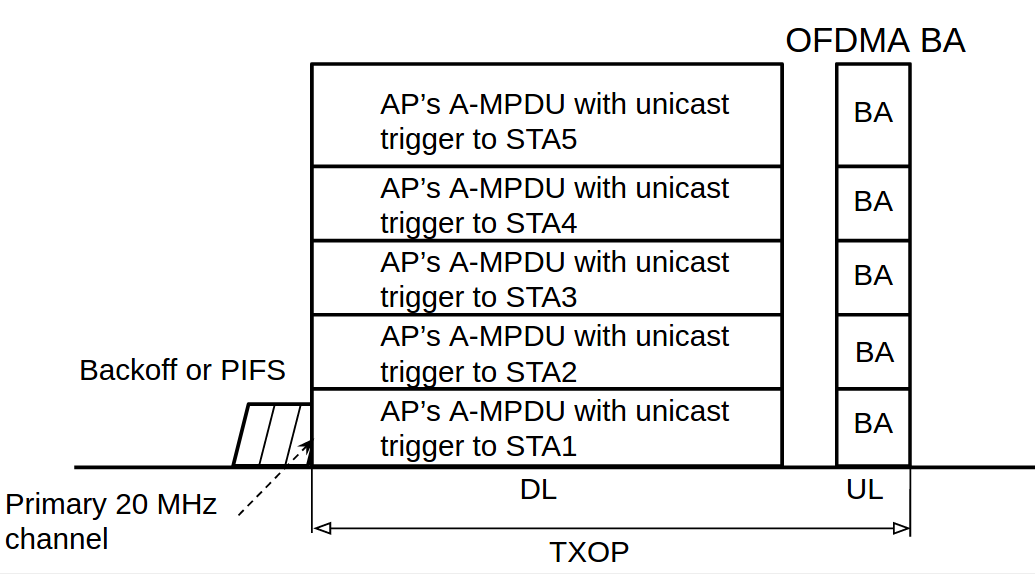
\includegraphics[scale=0.23]{./figure/fig_MU_DL.png}
\caption{MU DL of 802.11ax}
\label{fig_MU_DL}
\end{figure}


\begin{figure}[!t]
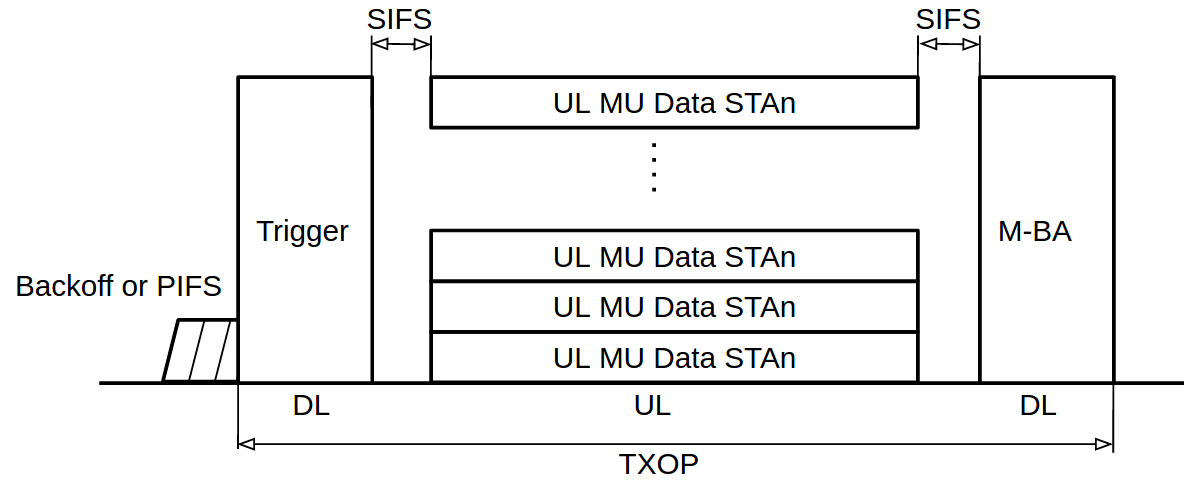
\includegraphics[scale=0.21]{./figure/fig_MU_UL.png}
\caption{Trigger-based MU UL of 802.11ax}
\label{fig_MU_UL}
\end{figure}

In respect of MAC layer, first for MU DL transmission, AP transmits DL packets to multiple stations simultaneously as in Fig. \ref{fig_MU_DL}.
Secondly, MU UL transmission is a little complicated as WiFi network is not a well-synchronized system, where preamble and acknowledgement mechanisms are required for a data packet transmission. 
A trigger-based MU UL transmission is thus issued as in Fig. \ref{fig_MU_UL}.
A brand new control frame, trigger frame (TF), is created to be transmitted by AP to initiate the UL transmission.
STAs could not transmit UL packets until they receive a TF which allocates RU for the STA or for random access. 
Afterwards, AP responds with ACK frame, forming a three-way handshake UL transmission. 
The trigger frame format is as in Fig. \ref{fig_TF_format}. 
Since the standard is in progress, some fields remain to be determined (TBD). 
In the field \textit{User Info}, subfield \textit{AID} represents the identification of STA and subfield \textit{RU Allocation} represents the RU allocated to the STA.
Especially, \textit{AID} with value 0 means the RU is for random access.


\begin{figure}[!t]
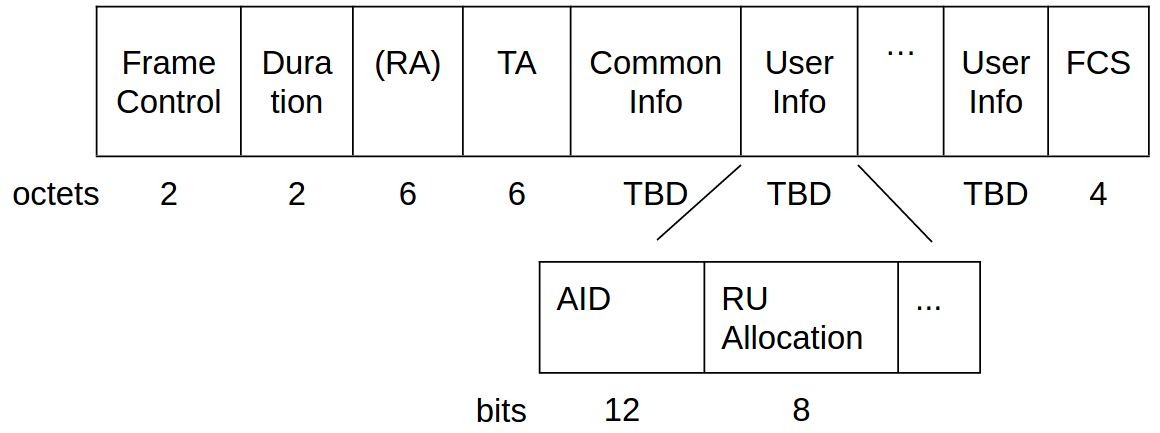
\includegraphics[scale=0.2]{./figure/fig_tf_format.png}
\caption{Trigger Frame format}
\label{fig_TF_format}
\end{figure}

%What's more, to support scheduling of TF, a mechanism called \textit{Target Wake Time} (TWT) is implemented in 802.11ax. TWT is originally issued in 802.11ah for power saving\cite{khorov2015survey}. It is also out of scope of this paper.



\subsection{OFDMA-based MCRA}		\label{sec_RA_illu}

\begin{figure*}[!ht]
\centering
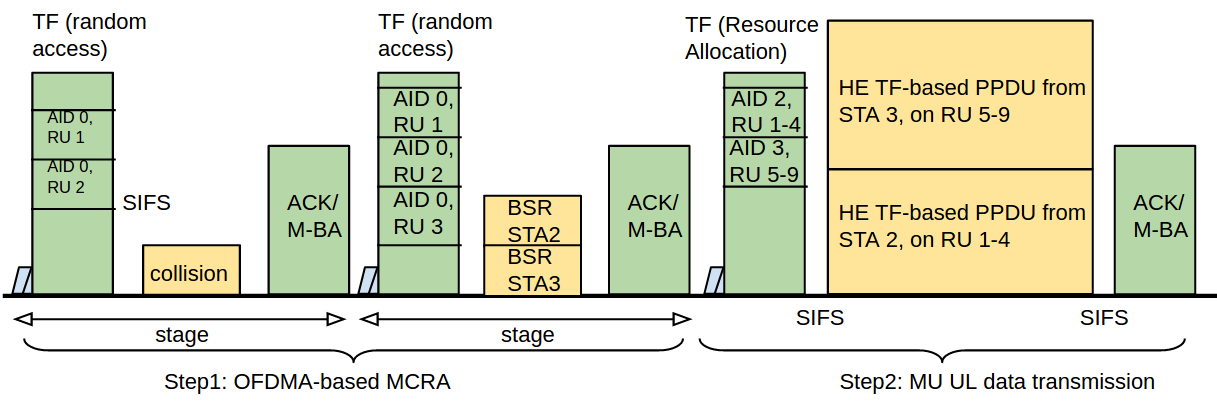
\includegraphics[scale=0.35]{./figure/RA_illu_4.png}
\caption{An example of Trigger-based MU UL transmission with OFDA-based MCRA}
\label{fig_ra_ul}
\end{figure*}


% 1. OFDMA-based MCRA is for UL
% 2. AP configure the parameters dynamically
% 3. TF-based MU UL above
% 4. detailed procedure of OFDMA-based MCRA

%Legacy IEEE 802.11 MAC is a 20 MHz SU PHY, which means that at most single user could succeed in contending at a time slot.
%With the MU PHY, HE-STA (802.11ax, high efficient station) has multiple RUs to access, which means multiple HE-STAs may access channel at the same time.
%And the parameter set is set by AP in real time.
%The procedure is of course more complicated and flexible.
%We first illustrate the ODFMA-based random access procedure then give two use cases of the random access.
An example of TF-based MU UL transmission with OFDMA-based MCRA, illustrated as in Fig. \ref{fig_ra_ul}, is divided into two steps, one as random access procedure and the other UL data transmission.
Random access procedure, namely the OFDMA-based MCRA, works as collecting traffic information from stations.
Thereby in the next step, AP could allocate RUs to STAs by transmitting a TF containing RU allocation.
Then the STAs, receiving the TF with resource allocation information, transmit UL data packets. And AP at last responds ACK.
Therefore, TF above in the example have two variants, one for random access and the other for resource allocation. 
The key of this mechanism locates at random access, i.e., the OFDMA-based MCRA, which is our concern.

\begin{figure}[!h]
%\begin{minipage}{.5\textwidth}
\centering
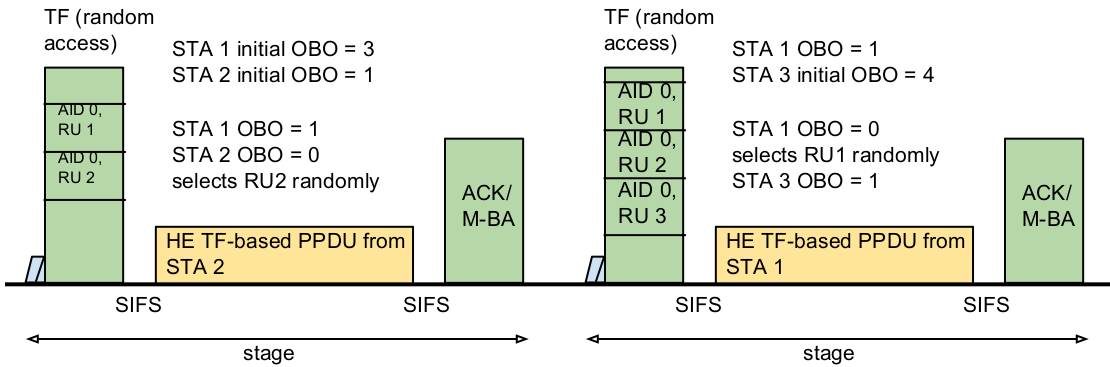
\includegraphics[scale=0.26]{./figure/RA_illu.png}
\caption{Illustration of OFDMA-based MCRA}
\label{fig_ra_illu}
%\end{minipage}
\end{figure}
Details of OFDMA-based MCRA mechanism is as Fig. \ref{fig_ra_illu}. 
To initialize a random access procedure, AP first transmits a TF announcing RUs for random access by setting the AID of the RUs to 0. 
Attempting STAs, whose buffers are not empty, maintain a backoff counter named OFDMA Backoff (OBO), which are randomly generated among range $[0, OCW]$.
Then the OBO subtracts the value of $M$ once receiving the TF, otherwise freezes, where $M$ is calculated by sum the number of RUs whose AID equals 0.  
When the OBO reaches 0, the STA will randomly select a RU from those whose AIDs equal 0 to transmit a request after short inter-frame spacing (SIFS). 
After that, AP responds with a block-ACK indicating which STAs contend successfully. The period of the whole three-way handshaking is named a \textit{stage}.
A successful stage means at least one STA contend successfully to transmit a request in a stage. 
It is worth noting that the stage in this paper, which is specified from standard \cite{draft_ax}, is a concept of the time interval, not the backoff stage in other papers.
To avoid confusion of the two meanings, backoff stage is replaced with \textit{backoff level} in this paper.  
When STAs fail to contend, the $OCW$ will be doubled until $OCW$ reaches $OCW_{max}$, which means the backoff level increases one step once a failure until the highest level.

In terms of implementation, system parameters of the MCRA are configured dynamically by AP, including $OCW_{min}, OCW_{max}, M$, where $OCW_{min}, OCW_{max}$ represent the minimum and the maximum contention window, and $M$ as the number of RUs for random access. 
Two of critical parameters $OCW_{min}, OCW_{max}$ are configured in Random Access Parameter Set (RAPS) element contained in beacon frame sent by AP.
Check field \textit{OCW Range} in RAPS element as in Fig. \ref{fig_RAPS}, $OCW_{min} = 2^{EOCW_{min}}-1$, $OCW_{max} = 2^{EOCW_{max}}-1$. 
$M$ is obtained from TF by sum the number of RUs whose \textit{AID} equal 0.
To simplify following analysis, we issue another parameter $m$, \textit{maximum backoff level}, so that $OCW_{max} = (OCW_{min}+1)*2^m-1$. 
The configuration of system parameter is absolutely different from that of legacy 802.11, where all the parameters are predefined in each STA's hardware. 
OFDMA-based MCRA is thus more flexible compared with DCF.



%Another use case of random access is for power save HE-STA to solicit buffered packets at AP, which is kind of DL transmission.
%Similar to legacy 802.11 power save, HE-STA needs to transmit PS-poll or APSD-trigger frame to inform AP of its active state when the HE-STA wakes up.
%The transmission of PS-poll or APSD-trigger frame is a good case of OFDMA-based random access. After successful contention, AP will transmit the buffered packets of the HE-STA.

\begin{figure}[!h]
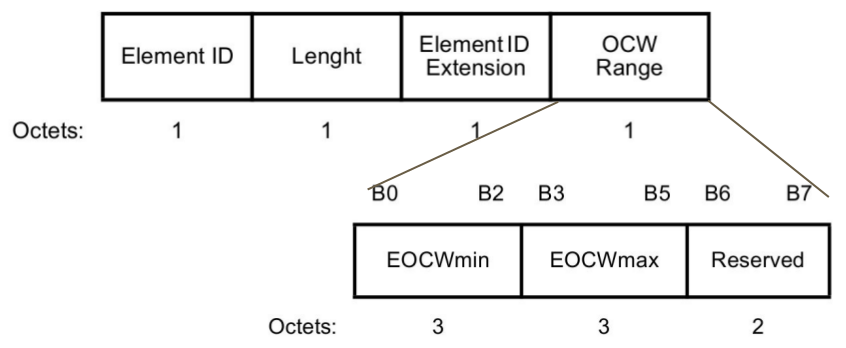
\includegraphics[scale=0.3]{./figure/RAPS.png}
\caption{Random Access Parameter Set (RAPS) Element}
\label{fig_RAPS}
\end{figure}



\section{System Model} 		\label{sec_sys_model}
Bianchi's Markov chain model has been validated that it accurately depicts the steady state behavior of DCF based on the assumption that at each request transmission, and regardless of the number of retransmission suffered, each request frame collides with constant and independent probability $p$. 
Although some differences exist between OFDMA-based MCRA and DCF, we have validated that OFDMA-based MCRA could be modeled with Markov chain model.

The analysis is divided into two parts. First is the Markov chain model to estimate the packet transmission probability $\tau$ and conditional collision probability $p$. 
Secondly, we evaluate some metrics given $\tau$, including the number of stations who succeed in contending in a stage $n_s$, self-defined system efficiency \textit{eff}, and expected access delay of a STA $D$.  
Table \ref{table_notation} is a list of all parameters and notations.


\begin{table}[!h]
\caption{Parameters and Notations Interpretation}
\centering
\label{table_notation}
\begin{tabular}{c|m{4.5cm}}
\hline
Notations				& Meaning \\
\hline
$n$						& Number of stations \\
$OCW_{min}$ ($W_0$)		& Minimum OFDMA contention window \\
$OCW_{max}$ ($W_m$)		& Maximum OFDMA contention window \\
$M$						& Number of RUs for random access \\
$m$						& Maximum backoff level \\
$p$						& Packet collision probability \\
$\tau$					& Station's transmission probability \\
$n_s$					& Number of successful stations in a stage \\
$D$						& Access delay, number of stages for a station to contend successfully \\
\hline
\end{tabular}
\end{table}

\subsection{Packet Transmission Probability}
Consider a fixed number $n$ of stations under saturation condition, which means each station is an attempting station. 
For saturation analysis, stage of MCRA is one after another.
Also, the ideal channel is assumed so that collision happens only if more than one station transmits at the same RU.
Since the critical of the mechanism is OFDMA-based MCRA, only UL request transmission is concerned, while DL transmission and UL data transmission are not considered here. 

To model OFDMA-based MCRA with the discrete-time Markov chain model, the concept of time is supposed to be adapted. 
In DCF, time unit of the model corresponds with slot, while in OFDMA-based MCRA time unit of the model is stage, a three-way handshake. 
Thus the delay will be measured in the number of stages.

Similar to Bianchi's work, let $\lbrace s(t), b(t) \rbrace$ be the bi-dimension process, where $s(t)$ denotes the backoff level $(0,\cdots, m)$, and $b(t)$ denotes backoff counter $(0,\cdots, W_i)$.
With the discrete and integer time scale, $t$ and $t+1$ corresponds to beginnings of two consecutive stages.
$\lbrace b(t) \rbrace$ is not Markov process because the state of the current stage depends on the history of transmission instead of only the previous stage. 
The bi-dimensional process $\lbrace s(t),b(t) \rbrace$ is also a Markov chain.
The key assumption is still necessary that at each request transmission, and regardless of the number of retransmission suffered, each request frame collides with constant and independent probability $p$.
With the independence assumption, $p$ will be a constant. The Markov chain is able to be conducted as in Fig. \ref{Markov}.

% Differences
Another important difference between the two Markov chain models of OFDMA-based MCRA and DCF, is clarified here.
Since the station of DCF senses the carrier before transmitting, it will freeze its backoff counter and stay at the state if channel is sensed busy. 
However in the OFDMA-based MCRA, because the time unit, a stage, contains a period for exactly a packet transmission, stations certainly subtract $M$ from the OBO only if they receive a TF for random access. 
Stations of the MCRA thus stay in one state for a period of exactly single stage.

% modifications
Some modifications are mentioned here to adapt to differences between OFDMA-based MCRA and DCF. 
First, in a row of states, as OBO subtracts the value of $M$ rather than $1$, stations transfer to states $M$-step ahead.
Second, since states with $b(t)\leq M $ will decrease to $0$ at the current state, which means stations could access RUs, we could merge these states into one state, denoted by $\lbrace i, T \rbrace$. $T$ is an integer set of $[0,M]$. 

\begin{figure*}[!t]
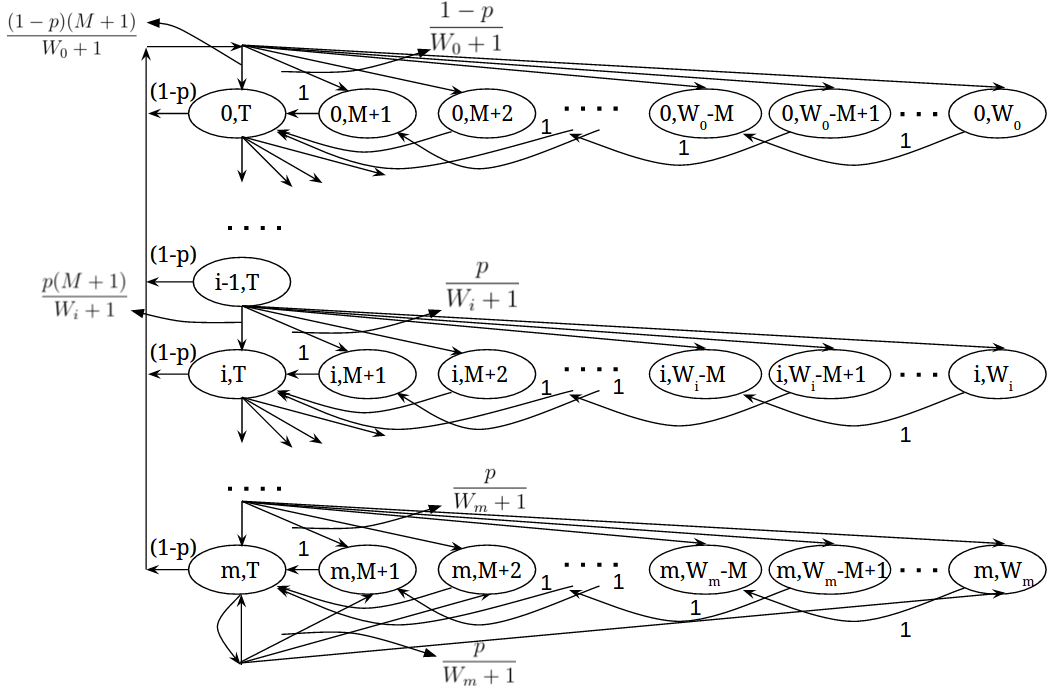
\includegraphics[scale=.45]{./figure/Markov_chain.png}
\caption{Markov Chain model for the backoff window size}
\label{Markov}
\end{figure*}

Let's assume $P\lbrace i_1, k_1|i_0,k_0\rbrace = P\lbrace s(t+1) = i_1, b(t+1)= k_1|s(t) = i_0, b(t) = k_0\rbrace $. In this Markov Chain, the only non null one-step transition probabilities are 
\begin{align}
\left\lbrace
\begin{array}{lll}
P\lbrace i, T | i, k \rbrace = 1  						& k\in [M+1,2M]			& i \in [0,m]\\ [3pt]
P\lbrace i, k-M | i, k \rbrace = 1  					& k\in [2M+1,W_i]   	& i \in [0,m]\\ [3pt]
P\lbrace 0, k | i, T \rbrace = \frac{1-p}{W_0+1}  		& k\in [M+1,W_0]		& i \in [0,m]\\ [3pt]
P\lbrace 0, T | i, T \rbrace = \frac{(1-p)(M+1)}{W_0+1} &						& i \in [0,m]\\ [3pt]
P\lbrace i, k | i-1, T \rbrace = \frac{p}{W_i+1} 		& k\in [M+1,W_i] 		& i \in [1,m]\\ [3pt]
P\lbrace i, T | i-1, T \rbrace = \frac{p(M+1)}{W_i+1}   &	  					& i \in [1,m]\\ [3pt]
P\lbrace m, k | m, T \rbrace = \frac{p}{W_m+1} 		 	& k\in [M+1,W_m] 		& \\ [3pt]
P\lbrace m, k | m, T \rbrace = \frac{p(M+1)}{W_m+1}
\end{array}
\right.
\label{trans_prob}
\end{align}

The first and second equations in (\ref{trans_prob}) accounts for the fact that the backoff counter maintained by stations will subtract $M$, the number of RUs for random access. 
The third and fourth equations represent that after a successful contention, stations will reset the contention window size to initial window size and uniformly generate a backoff value among $[0,W_0]$, since $T$ is an integer set $[0,M]$, the transition probability to states $\lbrace i, T \rbrace$ is $M+1$ times of that to states $\lbrace i, k \rbrace$. 
For the fifth and sixth equations, they represent when a failure contention occurs, the contention window size will be doubled, $W_i=2W_{i-1}+1$.
The last two equations are the case of failure at the maximum backoff level. 
We assume no packets are discarded, repeating retransmitting until success.

Let $b_{i,k} = \lim_{t\rightarrow \infty} P\lbrace s(t) = i, b(t) = k\rbrace,\ i\in [0,m], \ k \in [0,W_i]$, be the stationary distribution of the Markov chain. 
Then we show how to obtain transmission probability $\tau$ and conditional collision probability $p$.
First,  for states with $b(t) = T$, in which stations will transmit requests or BSRs in current stage, 
\begin{align}
b_{i-1,T}\cdot p = b_{i,T} 		\rightarrow b_{i,T} = p^i b_{0,T}, \quad 0\leq i < m \nonumber\\
b_{m-1,T}\cdot p = (1-p) b_{m,T}	\rightarrow b_{m,T} = \frac{p^m}{1-p}b_{0,T}.
\label{biT}
\end{align}

Then, other states are expressed with states in which $b(t)=T$:
\begin{align}
&b_{i,k} =  \nonumber \\
&
\begin{cases}
(\lfloor \frac{W_0-k}{M} \rfloor+1)\frac{(1-p)}{W_0+1}\sum_{i=0}^m b_{i,T}, \  M+1\leq k\leq W_0,\ i = 0\\[3pt]
(\lfloor \frac{W_i-k}{M} \rfloor+1)\frac{p}{W_i+1}b_{i-1,T}, 				\	 M+1 \leq k\leq W_i, \ 0<i<m \\[3pt]
(\lfloor \frac{W_m-k}{M} \rfloor+1)\frac{p}{W_m+1} (b_{m-1,T}+b_{m,T}), 	
\end{cases}\nonumber
\\ &\qquad \qquad \qquad \qquad \quad \qquad \qquad M+1 \leq k\leq W_m, \quad i = m \nonumber \\
\label{steady_prob}
\end{align}

From (\ref{biT}), $\sum_{i=0}^m b_{i,T}= \frac{b_{0,T}}{1-p}$ is obtained; whereby (\ref{steady_prob}) could be summed respectively to get (\ref{part_sum}).  

\begin{figure*}[!t]
\begin{align}
\begin{cases}
\sum_{k=M+1}^{W_0} b_{0,k} = \frac{b_{0,T}}{W_0+1}\left(-\frac{M}{2}\left\lfloor \frac{W_0}{M}\right\rfloor ^2 + \left(W_0-\frac{M}{2}\right)\left\lfloor \frac{W_0}{M} \right\rfloor \right) \\[8pt]
\sum_{i=1}^{m-1}\sum_{k=M+1}^{W_i} b_{i,k} = \frac{b_{0,T}}{W_0+1}\left(\frac{p}{2}\right)^i \left(-\frac{M}{2}\left\lfloor \frac{W_i}{M}\right\rfloor ^2 + \left(W_i-\frac{M}{2}\right)\left\lfloor \frac{W_i}{M} \right\rfloor \right) \\[8pt]
\sum_{k=M+1}^{W_m} b_{m,k} = \frac{b_{0,T}}{W_0+1}\frac{(\frac{p}{2})^m}{1-p}\left(-\frac{M}{2}\left\lfloor \frac{W_m}{M}\right\rfloor ^2 + \left(W_m-\frac{M}{2}\right)\left\lfloor \frac{W_m}{M} \right\rfloor \right) 
\end{cases}
\label{part_sum}
\end{align}
\end{figure*}

Each subequation in (\ref{part_sum}) has the same term: $-\frac{M}{2}\left\lfloor \frac{W_i}{M}\right\rfloor ^2 + \left(W_i-\frac{M}{2}\right)\left\lfloor \frac{W_i}{M} \right\rfloor$. 
To simplify the expression, let $X_i = -\frac{M}{2}\left\lfloor \frac{W_i}{M}\right\rfloor ^2 + \left(W_i-\frac{M}{2}\right)\left\lfloor \frac{W_i}{M} \right\rfloor$. 
Then, sum the steady state probability of all states to get (\ref{total_sum2}).

\begin{figure*}[!t]
\begin{align}
1 &= \sum_{i=0}^m \sum_{k=0}^{W_i}b_{i,k} 
 = \frac{b_{0,T}}{W_0+1}\left( X_0 + \sum_{i=1}^{m-1}X_i\left( \frac{p}{2}\right)^i + X_m\frac{\left( \frac{p}{2}\right)^m}{1-p}\right) + \frac{b_{0,T}}{1-p}\label{total_sum}\\
& = b_{0,T}\left( \frac{(1-p)X_0+(1-p) \sum_{i=1}^{m-1}X_i\left( \frac{p}{2}\right)^i+X_m\left( \frac{p}{2}\right)^m+W_0+1}{(W_0+1)(1-p)}\right), \label{total_sum2}
\end{align}
%\setcounter{equation}{7}%{\value{MYtempeqncnt}}
%% IEEE uses as a separator
\hrulefill
\end{figure*}

whereby a closed-form expression of $\tau$, the probability of a station transmitting a request at a stage, is derived.

\begin{align}
\label{tau_general}
&\tau = \sum_{i=0}^m b_{i,T} = \frac{b_{0,T}}{1-p} = \nonumber \\
&\frac{W_0+1}{W_0+1+(1-p)X_0+(1-p) \sum_{i=1}^{m-1}X_i\left( \frac{p}{2}\right)^i+X_m\left( \frac{p}{2}\right)^m}
\end{align}

For $m=0, M=1$ which is SU PHY with a fixed contention window, check (\ref{total_sum}), the terms containing $X_i, i>0$ will disappear, and $b_{0,T}/(1-p)$ degrades to $b_{0,T}$.
As a result, (\ref{total_sum2}) degrades to 
\begin{align}
1 = b_{0,T}\left( \frac{W_0+1+X_0}{W_0+1}\right).
\end{align}
Thereby, 
\begin{align}
\tau = b_{0,T} &= \frac{W_0+1}{W_0+1+X_0} \nonumber\\
				&= \frac{2(W_0+1)}{W_0^2+W_0+2},
\label{tau_W0}
\end{align}
which is different from that of CSMA/CA with constant window size \cite{ho1996performance}, where $\tau=\frac{2}{W_0+1}$.
That is because stations of CSMA/CA freezes backoff counter when sensing busy channel while no such freeze mechanism of backoff counter exists in OFDMA-based MCRA. 


On the other hand, conditional collision probability $p$ has another relation with the probability $\tau$. 
With ideal channel assumption that the collision happens only if at least one of other stations select the same RU, we have 
\begin{align}
\label{p_ax}
p = 1-\left( 1-\frac{\tau}{M} \right)^{n-1}.
\end{align}
Rewrite (\ref{p_ax}) as $\tau^\star = \left(1-(1-p)^\frac{1}{n-1} \right)M$. 
To obtain probability $\tau$ and $p$, we need to find solutions to a group of the two equations \ref{tau_general} and \ref{p_ax}.
$\tau^\star(p)$ is a monotonically increasing function. 
Though $\tau(p)$ is hard to determine the monotonicity from the expression of equation \ref{tau_general} with respect to $p$, the  function \ref{tau_general} is estimated monotonically decreasing by numerical method. 
Also, $\tau(0) = \frac{W_0+1}{W_0+1+X_0}> \tau^\star(0) = 0$.
And $\tau(1) < \tau^\star(1) = M$. 
Therefore, the only solution could be found by numerical method.



\subsection{Random Access Efficiency}
With the transmission probability $\tau$, performance of OFDMA-based MCRA mechanism could be easily evaluated. 
First, the expected number of stations who contend successfully at a stage, denoted by $E[n_s]$. 
Extending $n_s$, a system efficiency is defined as another important metric.
Also, the access delay denoted by $D$, referred to as number of stages required for a station to contend successfully, could be derived. 

\subsubsection{$n_s$ and System Efficiency}
What we are concerned about is that how many stations contend successfully at a stage.
Given $\tau$ and $p$, the probability that a station contend successfully in a stage is firstly derived: $P_{s\_station} = \tau (1-p)$.
Then, with (\ref{p_ax}), $E[n_s]$ is easily expressed as follows. 
\begin{align}
\label{equ_ns}
E[n_s] &= n P_{s\_station} \nonumber \\
		&= n\tau (1-p) \nonumber \\
		&= n\tau (1-\frac{\tau}{M})^{n-1}
\end{align}

Furthermore, normalizing $n_s$, \textit{system efficiency} here is defined as the ratio of the number of successful contending stations in a stage to the number of RUs for random access in a stage.
\begin{align}
\label{eff_def}
\textit{eff}\ (\tau) &=\frac{E[n_s]}{M} \nonumber \\
					 &= \frac{n\tau(1-\frac{\tau}{M})^{n-1}}{M}
\end{align}


	
\subsubsection{Access Delay}
$D$ represents the number of stages required for a station to contend successfully in a stage. 
Because of saturation assumption, a new request arrives once one previous request is transmitted successfully.
Thus queueing waiting time is not considered here. 
In this way, the access delay $D$ follows the geometric distribution with parameter $P_{s\_station}$, which is obtained just now.  
Then the expected value of access delay of request frame, $E[D]$, is 
\begin{align}
\label{equ_delay}
E[D] = \frac{1}{\tau (1-\frac{\tau}{M})^{n-1}}.
\end{align}




\section{Model Validation} 		\label{sec_model_val}
The same with scenario for analysis, only OFDMA-based MCRA mechanism, i.e., Fig. \ref{fig_ra_illu}, is concerned.
Simulation runs with three-way handshake stage by stage.
We run simulations for 1,000,000 stages with a variety of parameter sets $\lbrace M, OCW_{min}, OCW_{max}\rbrace$ and collects the information of the two variables, the number of successful attempt STAs $n_s$ and expected access delay $D$. 
The values of results from both analysis and simulation are given in Fig. \ref{validation} and Table \ref{table_val}. 
The results show that the Markov model precisely predicts the steady state behavior of the OFDMA-based MCRA mechanism.

\begin{table}[!h]
\caption{Analysis versus simulation: $n_s$ and access delay with $m=3,M=9,OCW_{min} = 15$}
\label{table_val}
\begin{center}
\begin{tabular}{c|c|c}
\hline
$n_s$ 	& analysis 	& simulation \\
\hline
$n=1$ 	& 0.72727  	& 0.72728 \\
$n=5$ 	& 2.23001	& 2.22335 \\
$n=10$	& 2.88954	& 2.88546 \\
$n=20$	& 3.29798	& 3.29857 \\
\hline
delay	& analysis	& simulation \\
\hline
$n=1$ 	& 1.37500  	& 1.37499 \\
$n=5$ 	& 2.24214	& 2.24886 \\
$n=10$	& 3.46075	& 3.46565 \\
$n=20$	& 6.06432	& 6.06323 \\
\hline
\end{tabular}
\end{center}
\end{table}

%\input{validate.tex}

\begin{figure}[!h]
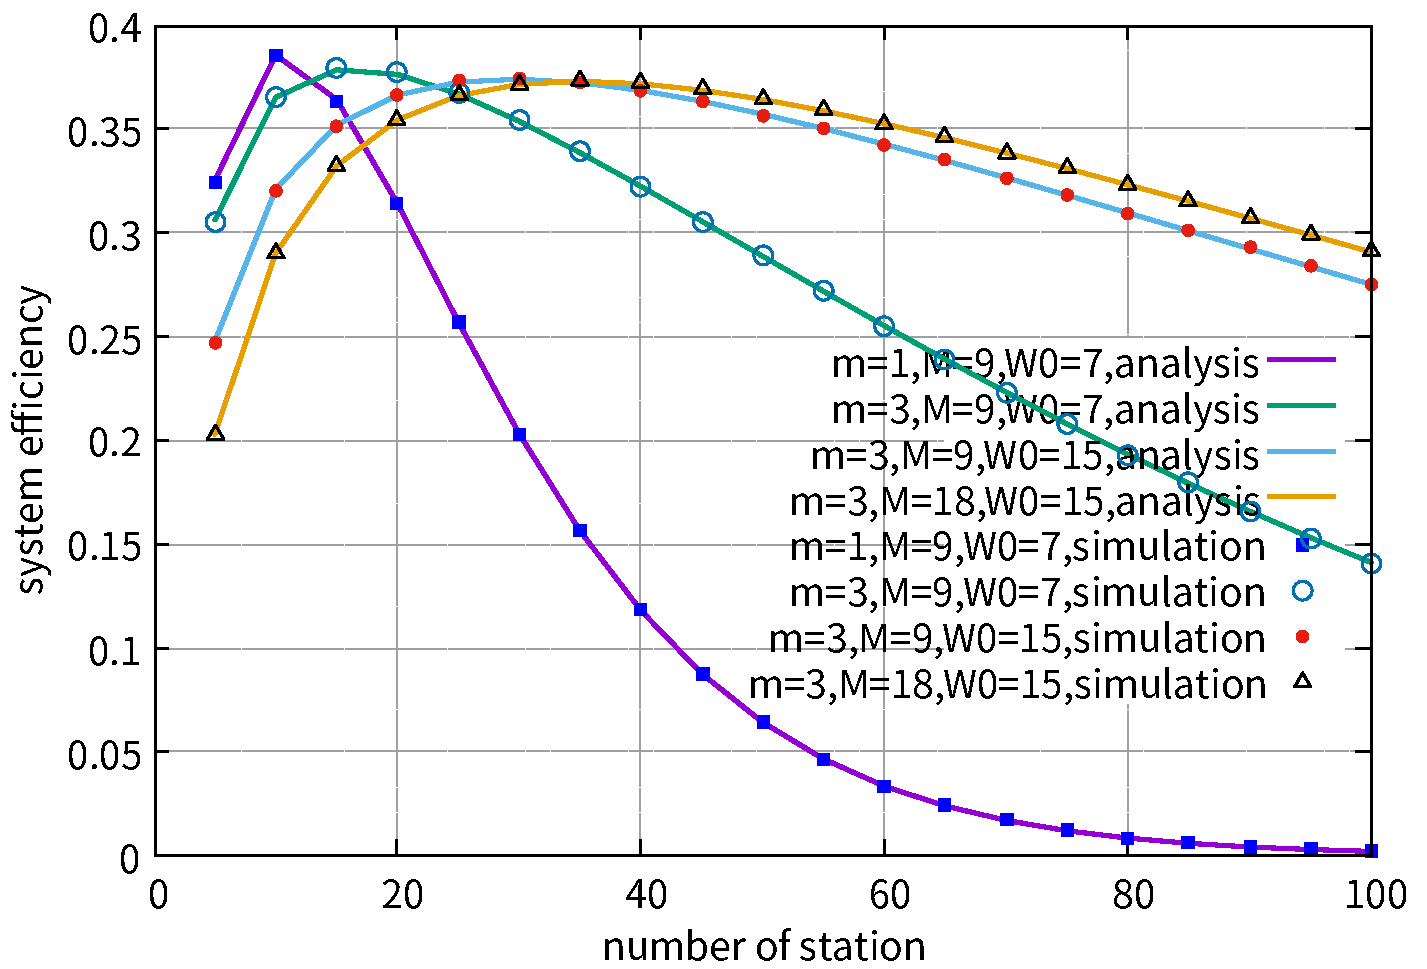
\includegraphics[scale=0.38]{./figure/Section_model_validate/validate.pdf}
\caption{System efficiency: Analysis versus Simulation}
\label{validation}
\end{figure}

\section{Performance Evaluation} 	\label{sec_perf_eval}

With above analysis, we could conveniently evaluate performance, including system efficiency and access delay, and the effects of system parameters.
Since the model acts quite precisely, model analysis is solicited to evaluate the performance later.

\subsection{Maximum System Efficiency and Minimum Access Delay} 	\label{sec_max_min}
With the system efficiency given in (\ref{eff_def}), take the derivative with respect to $\tau$, and find the extreme point, $\tau^\star = M/n$. Since $\tau\in [0,1]$, $\tau^\star = min\lbrace 1,M/n\rbrace$. 
In the dense scenario, i.e., $n$ is large, then $\tau^\star = M/n$. 
The system efficiency thus is
\begin{align}
\textit{eff}\ (\tau^\star) = (1-\frac{1}{n})^{n-1} 
\label{equ_max_eff}
\end{align}
Then the maximum $n_s$ is 
\begin{align}
\label{equ_max_ns}
E[n_s]^\star = M \cdot \textit{eff}\ (\tau^\star) = M(1-\frac{1}{n})^{n-1} .
\end{align}
The limit of system efficiency, based on infinite $n$, is
\begin{align}
\label{eff_limit}
\lim_{n\rightarrow \infty}\textit{eff}\ (\tau^\star) = \lim_{n\rightarrow \infty}(1-\frac{1}{n})^{n-1} =\frac{1}{e} 
\end{align}
which is the same with efficiency of SU slotted Aloha \cite{roberts1975aloha}.

%\begin{figure}[!ht]
%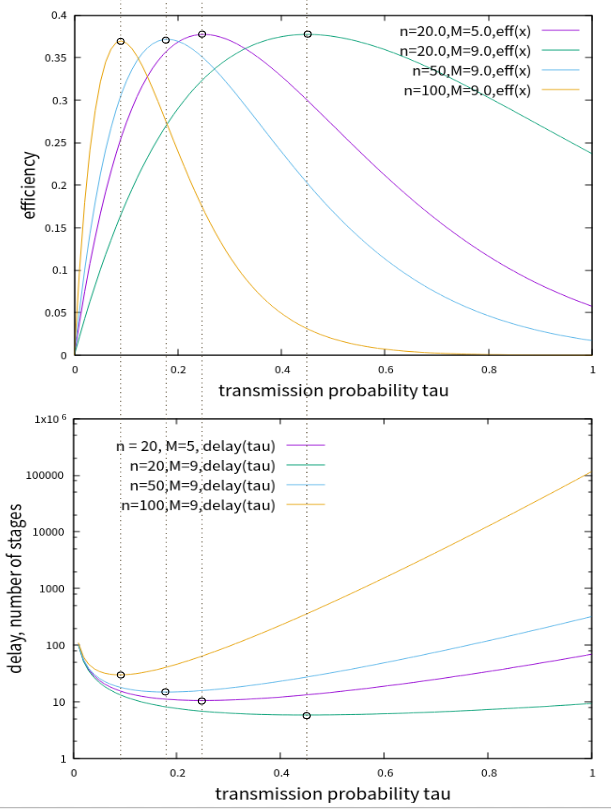
\includegraphics[scale=0.42]{./figure/chp4/max_min.png}
%\caption{Efficiency and access delay versus transmission probability $\tau$}
%\label{fig_eff_def}
%\end{figure}


With the delay analysis given in (\ref{equ_delay}), take the derivative with respect to $\tau$, and find the extreme point, $\tau^\star = M/n$. Also, $\tau^\star = min\lbrace 1, M/n\rbrace$. 
When $n\geq M$, the minimum access delay is  
\begin{align}
\label{equ_min_delay}
D(\tau^\star) = \frac{n}{M(1-\frac{1}{n})^{n-1}}.
\end{align}

From above analysis, we find that the maximum system efficiency and minimum access delay are both obtained by the $\tau^\star = min\lbrace 1, M/n\rbrace$.
What's more, optimal system efficiency is independent with $M$, while $M$ affects access delay. 
The larger $M$ is, the shorter the access delay will be. 
It indicates that when AP allocates RUs for random access, the AP could allocate as many as possible.

%Fig. \ref{fig_eff_def} is plotted in accordance with (\ref{eff_def}) and (\ref{equ_delay}).
%Consistent with the analysis above, the figure shows that the maximum system efficiency is independent of the number of RUs for random access when $n\geq M$, and approaching to $1/e$ with $n$ increasing. 
%What's more, the optimal transmission probability $\tau$ of system efficiency and access delay is consistent with each other, which also validates the analysis. 

Since $\tau$ and $p$ are obtained by solving group equations (\ref{tau_general}) and (\ref{p_ax}), it's hard to give a closed-form expression of $\tau$ only depending on system parameters, $M$, $W_0$, $m$ and $n$.
The only way to catch the insights of the MCRA is to tune the system parameters $\lbrace M, W_0, W_m \rbrace$ one by one.

\subsection{RUs for Random Access $M$}
\label{M}
(\ref{equ_max_eff}) has indicated that $M$, has nothing to do with optimal system efficiency. 
However, $n_s$ and $D$ are proportional and inversely proportional to $M$ respectively according to (\ref{equ_max_ns}) and (\ref{equ_min_delay}). 
Following analysis results validate the statement. 


\begin{figure}[!h]
\centering
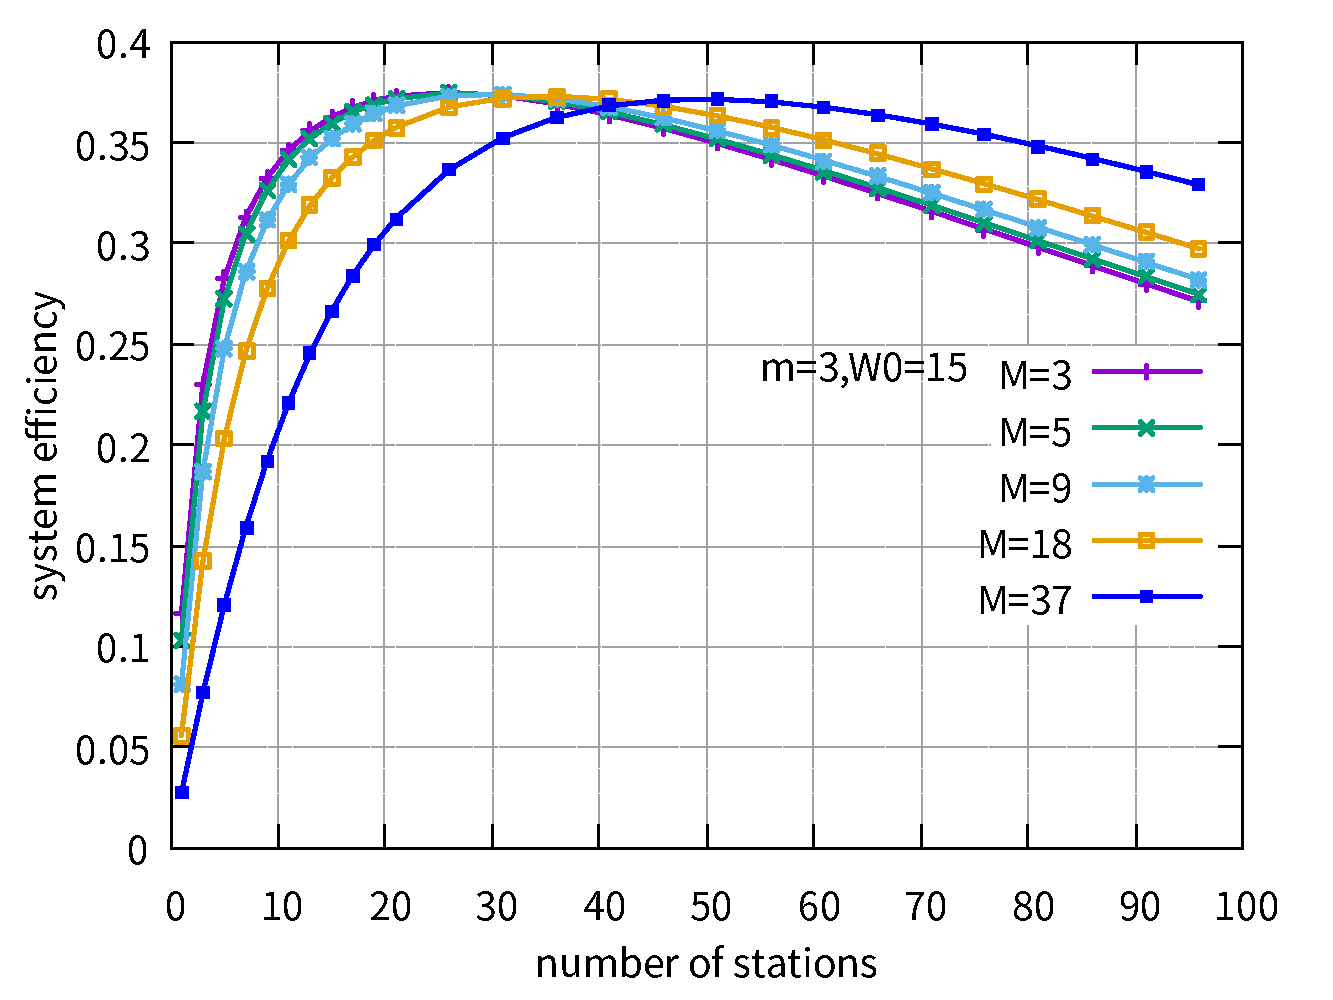
\includegraphics[scale=.38]{./figure/Section_perf_eval/M/n_M_eff_perf.pdf}
\caption{System efficiency versus number of stations}
\label{fig_n_M_eff}
\end{figure}

\begin{figure}[!h]
\begin{subfigure}{0.5\textwidth}  
%\centering
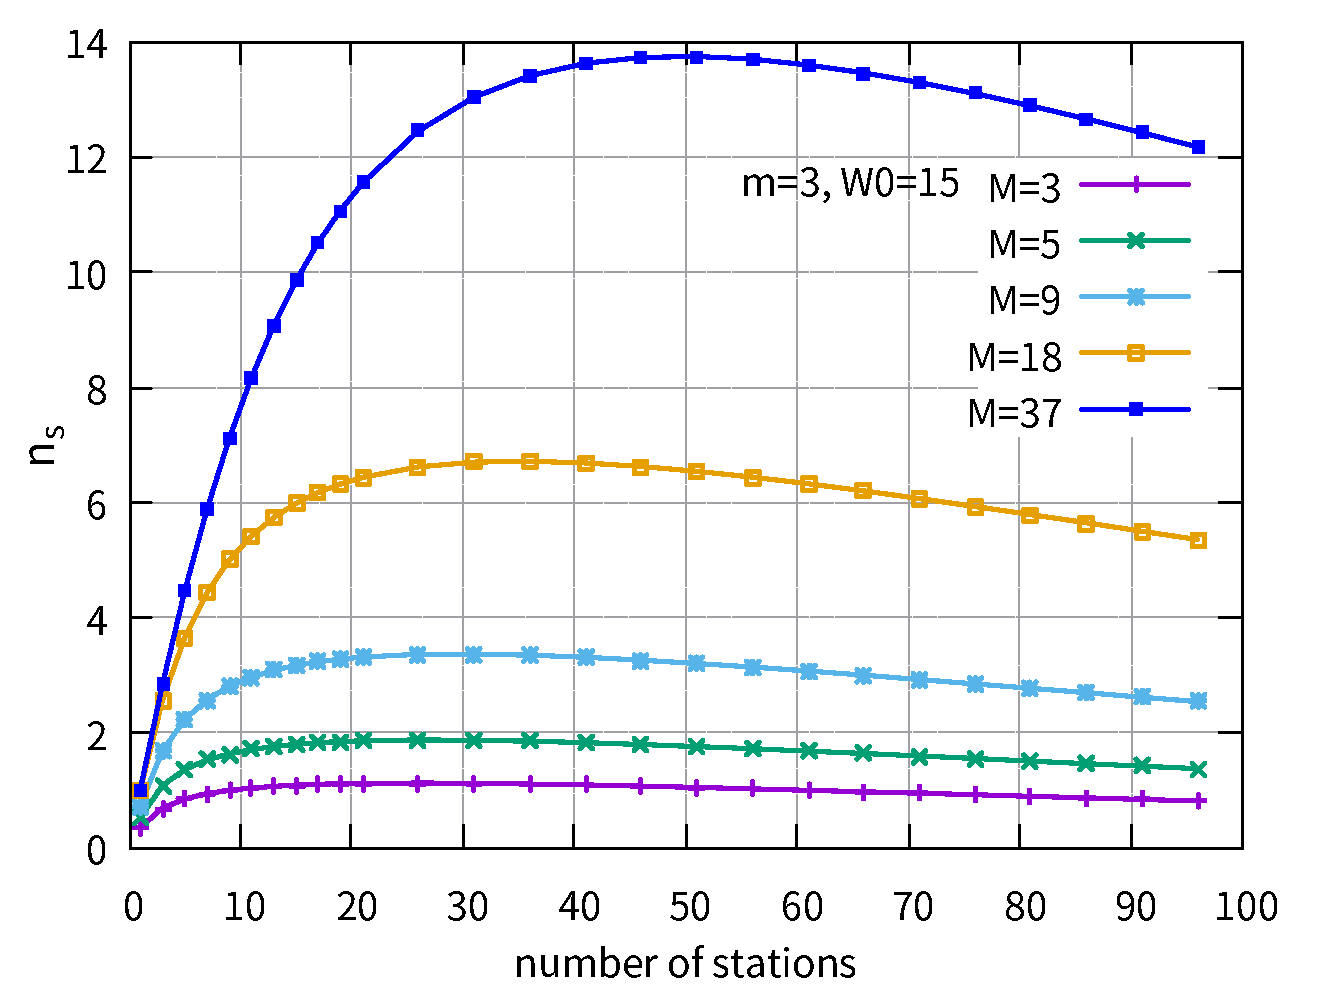
\includegraphics[scale=.38]{./figure/Section_perf_eval/M/n_M_ns_perf.pdf}
\caption{Number of successful stations in a single stage versus number of stations}
\label{fig_n_M_ns}
\end{subfigure}

\begin{subfigure}{0.5\textwidth}  
%\centering
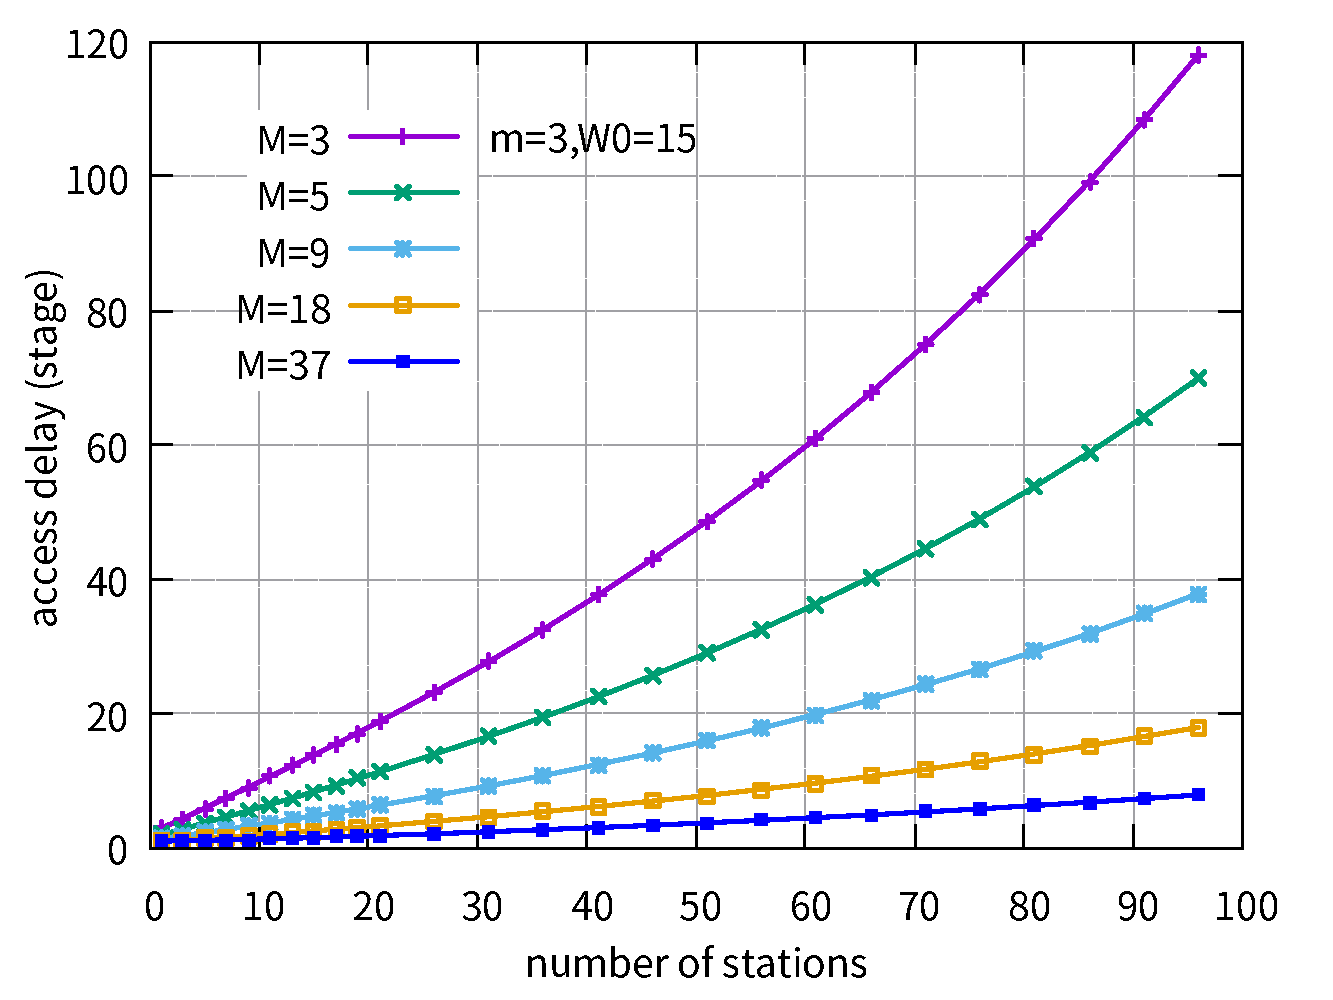
\includegraphics[scale=.38]{./figure/Section_perf_eval/M/n_M_delay_perf.pdf}
\caption{Access delay versus number of stations}
\label{fig_n_M_delay}
\end{subfigure}
\caption{Configure $M$}
\end{figure}

In Fig. \ref{fig_n_M_eff}, the maximum system efficiency from various cases are almost the same, approaching $1/e$. 
The only difference is "where" the optimal point locates. 
Practically, the other two metrics, $n_s$ and $D$, are closely related to $M$.
Fig. \ref{fig_n_M_ns} shows that larger $M$ results more stations contend successfully in a stage.
Moreover, Fig. \ref{fig_n_M_delay} shows that larger $M$ markedly decrease the access delay. 
Above all, when AP allocates RUs for random access, AP should allocate as many RUs as possible.



\subsection{$OCW_{min}, OCW_{max}$}
\label{contend_window}

% figures
\begin{figure}[!h]
\centering
%subfigure
\begin{subfigure}{0.5\textwidth}
%\centering
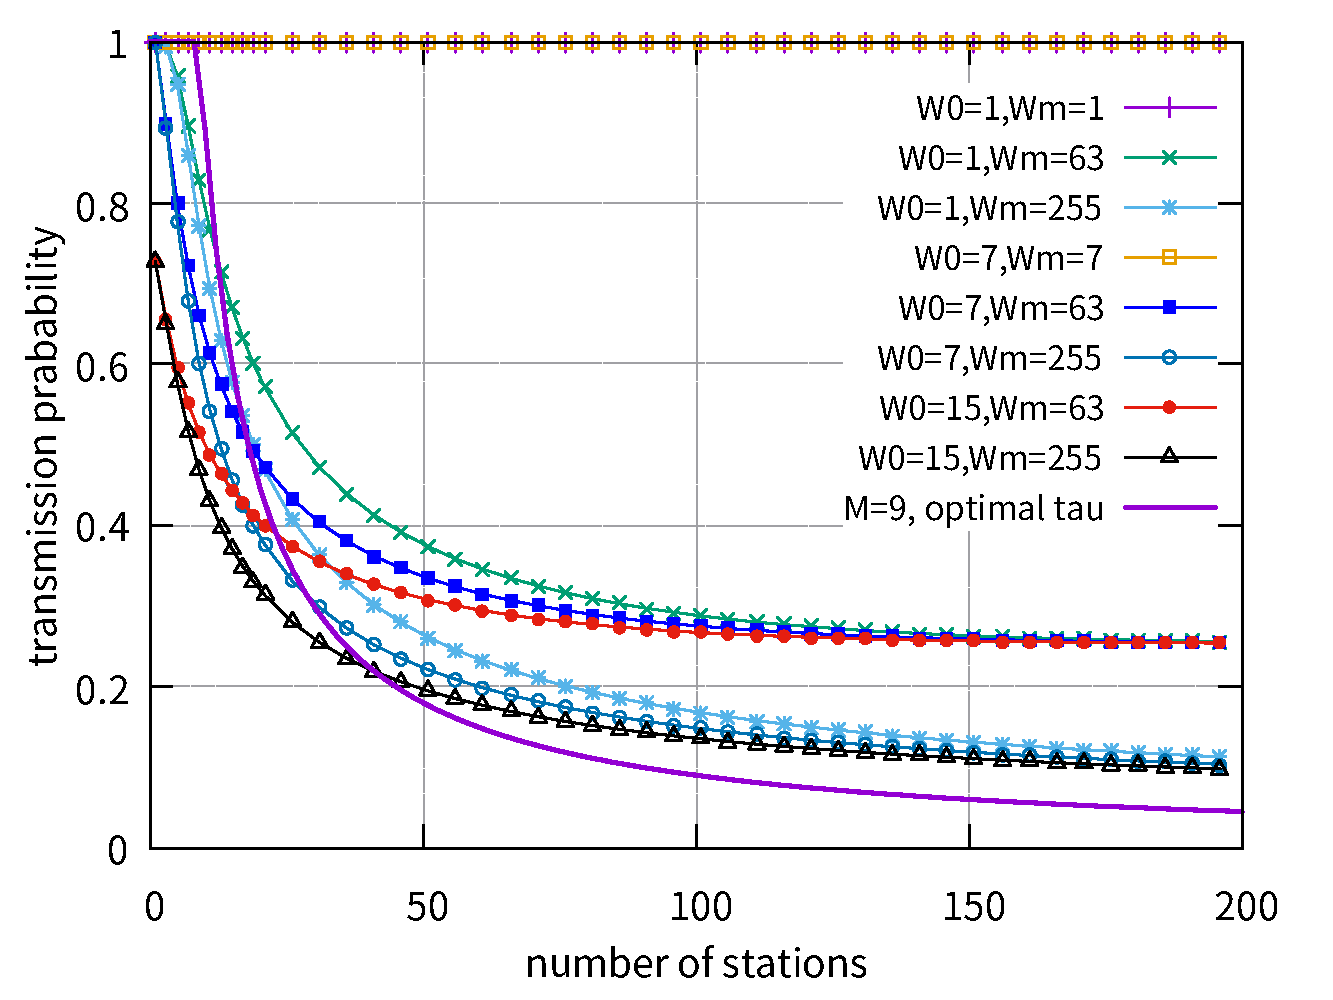
\includegraphics[scale=.38]{./figure/Section_perf_eval/tau/n_tau_perf_M9_x200.pdf}
\caption{Case 1, given $M=9$}
\label{fig_tau_n_M9}
\end{subfigure}
%subfigure
\begin{subfigure}{0.5\textwidth}
%\centering
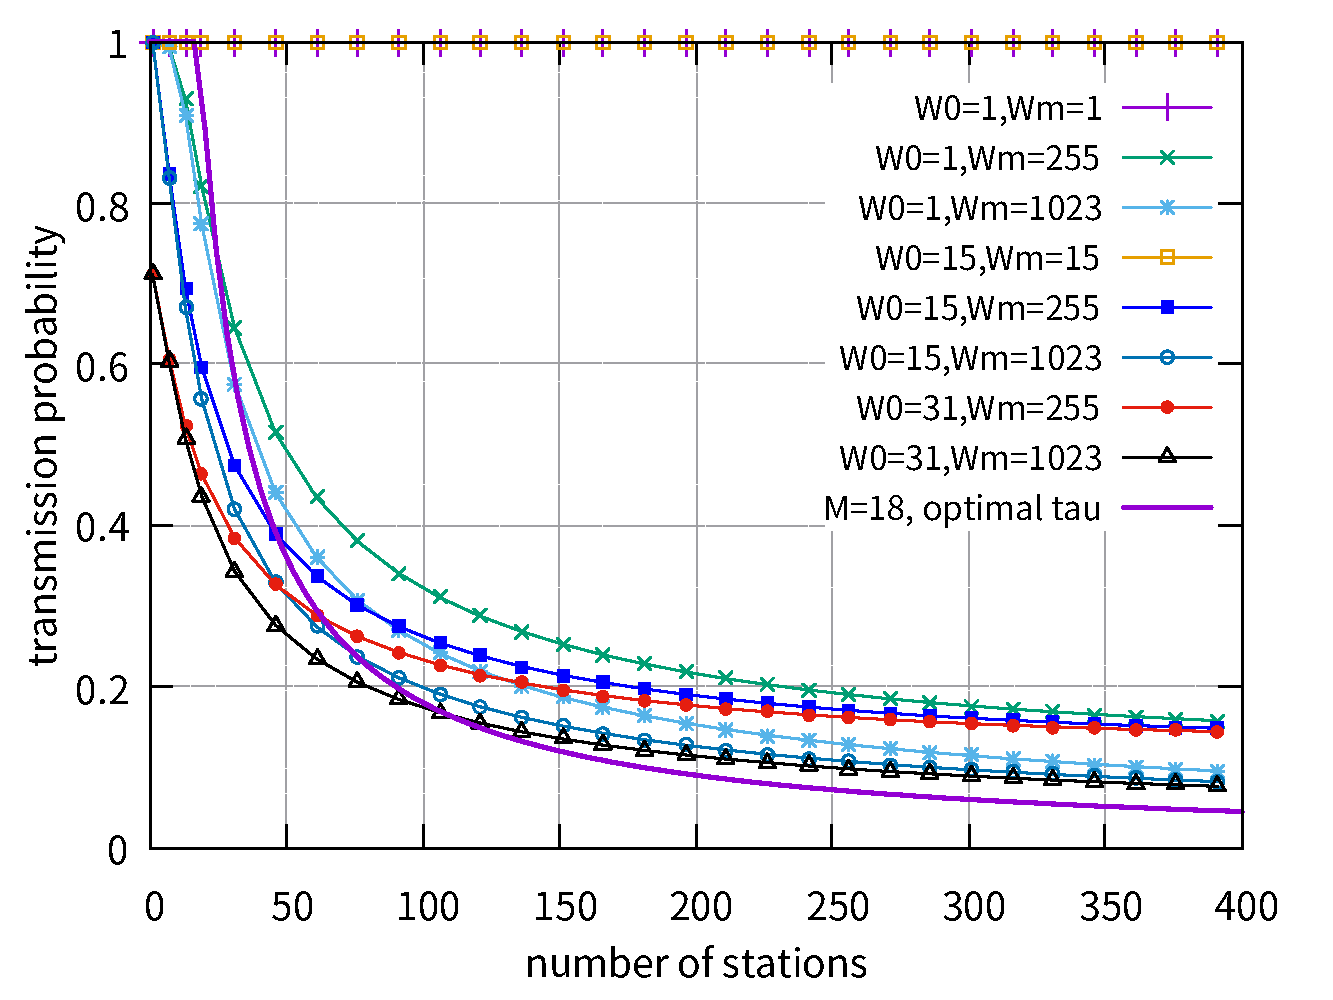
\includegraphics[scale=.38]{./figure/Section_perf_eval/tau/n_tau_perf_M18_x400.pdf}
\caption{Case 2, given $M=18$}
\label{fig_tau_n_M18}
\end{subfigure}
%caption
\caption{Transmission probability versus number of stations}
\label{fig_tau_n}
\end{figure}
% should have sth beginning
%For those $m>0$, the curve will be convex and monotone decreasing. It is intuitive that with the increasing number of stations, the transmit probability decreases.
Fig. \ref{fig_tau_n} shows case 1 ($M=9$) and case 2 ($M=18$), so that the rules we get are more convinced.
In the figure, the purple line without point depicts the $\tau^\star$ that $\tau^\star = min\lbrace 1, M/n \rbrace$.
With above analysis and effects of $M$, we tune remaining parameters $OCW_{min}, OCW_{max}$ so that $\tau$ approaches the optimal line. 
To see the trend of the line clearly, larger $n$ is configured so that some rules could be obtained as follows.

First, the $OCW_{min}$ or $W_0$, determines $\tau$ with small $n$. 
The larger $W_0$ is, the lower $\tau$ is at $n=1$.
That's why cases in Fig. \ref{fig_tau_n} have two different start points.

Secondly, $m=0$ results in constant $\tau$, which is consistent with (\ref{tau_W0}) that $\tau$ does not depend on $n$.
A special case, $W_0<M$ for scenario $n\leq M$, results in constant $\tau$ equals to 1 regardless of $n$. 
It perfectly matches $\tau^\star$ at $n\leq M$ as $\tau^\star = 1$ for the scenario $n \leq M$.
Thus, if given $n\leq M$, the optimal configuration will be $OCW_{max}= OCW_{min} < M$. 


Thirdly, performance of the dense scenario strongly depends on $OCW_{max}$.
It determines the limit of the $\tau$, i.e., where the line of $\tau$ will converge. 
And both the two figures in Fig. \ref{fig_tau_n} correspond with the above statement.
And larger $W_m$ causes lower $\tau$, which is closer to $\tau^\star$ when $n$ is large. 


% figures
\begin{figure}[!h]
\centering
\begin{subfigure}{0.5\textwidth}
\centering
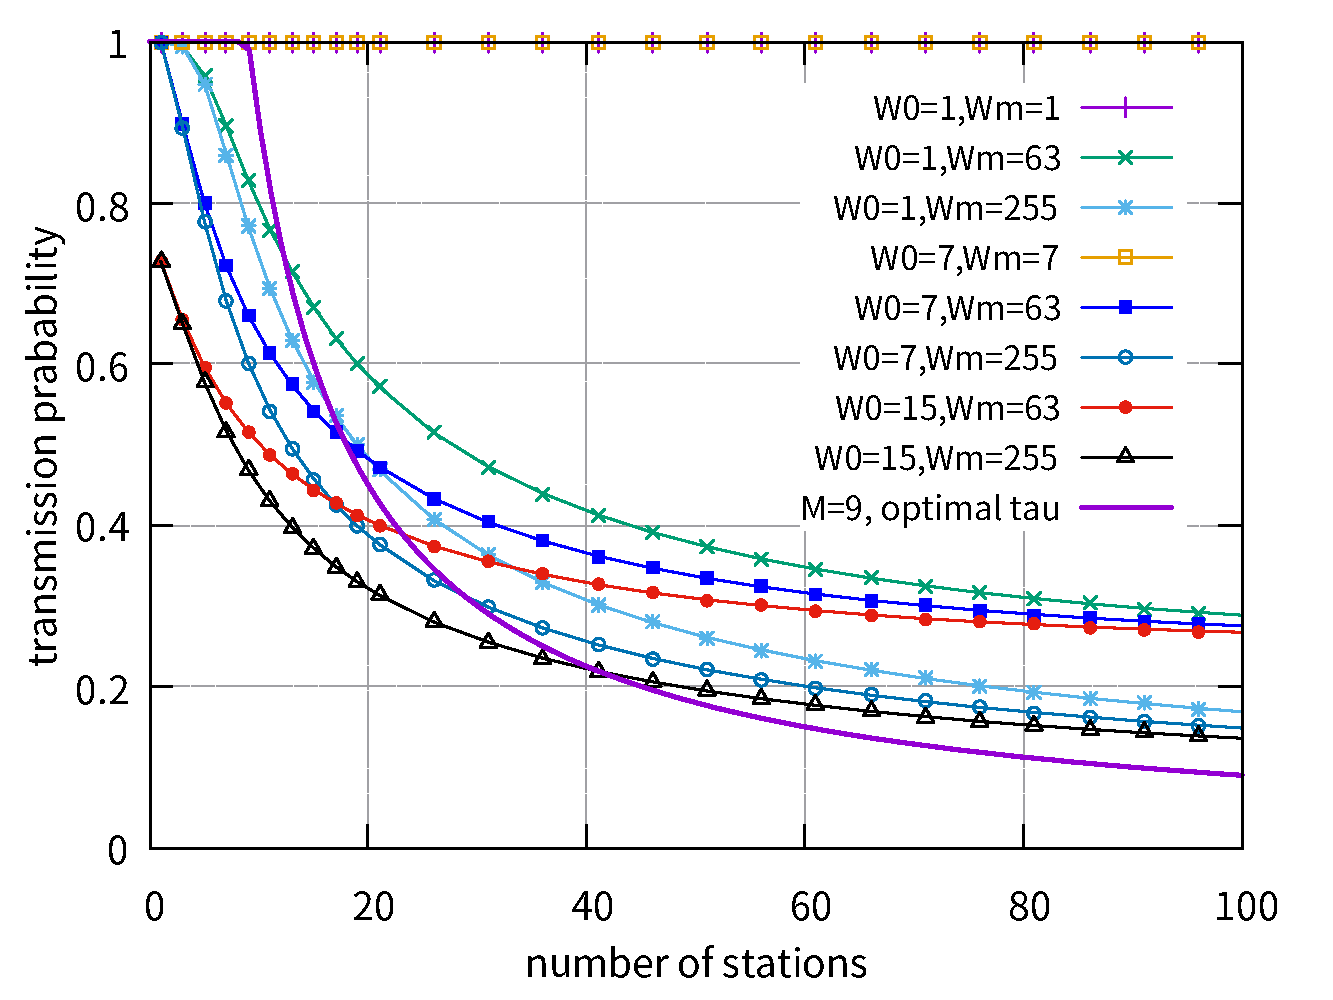
\includegraphics[scale=.38]{./figure/Section_perf_eval/tau/n_tau_perf_M9_x100.pdf}
\caption{Case 1, given $M=9$}
\label{fig_tau_n_M9_detail}
\end{subfigure}

\begin{subfigure}{0.5\textwidth}
\centering
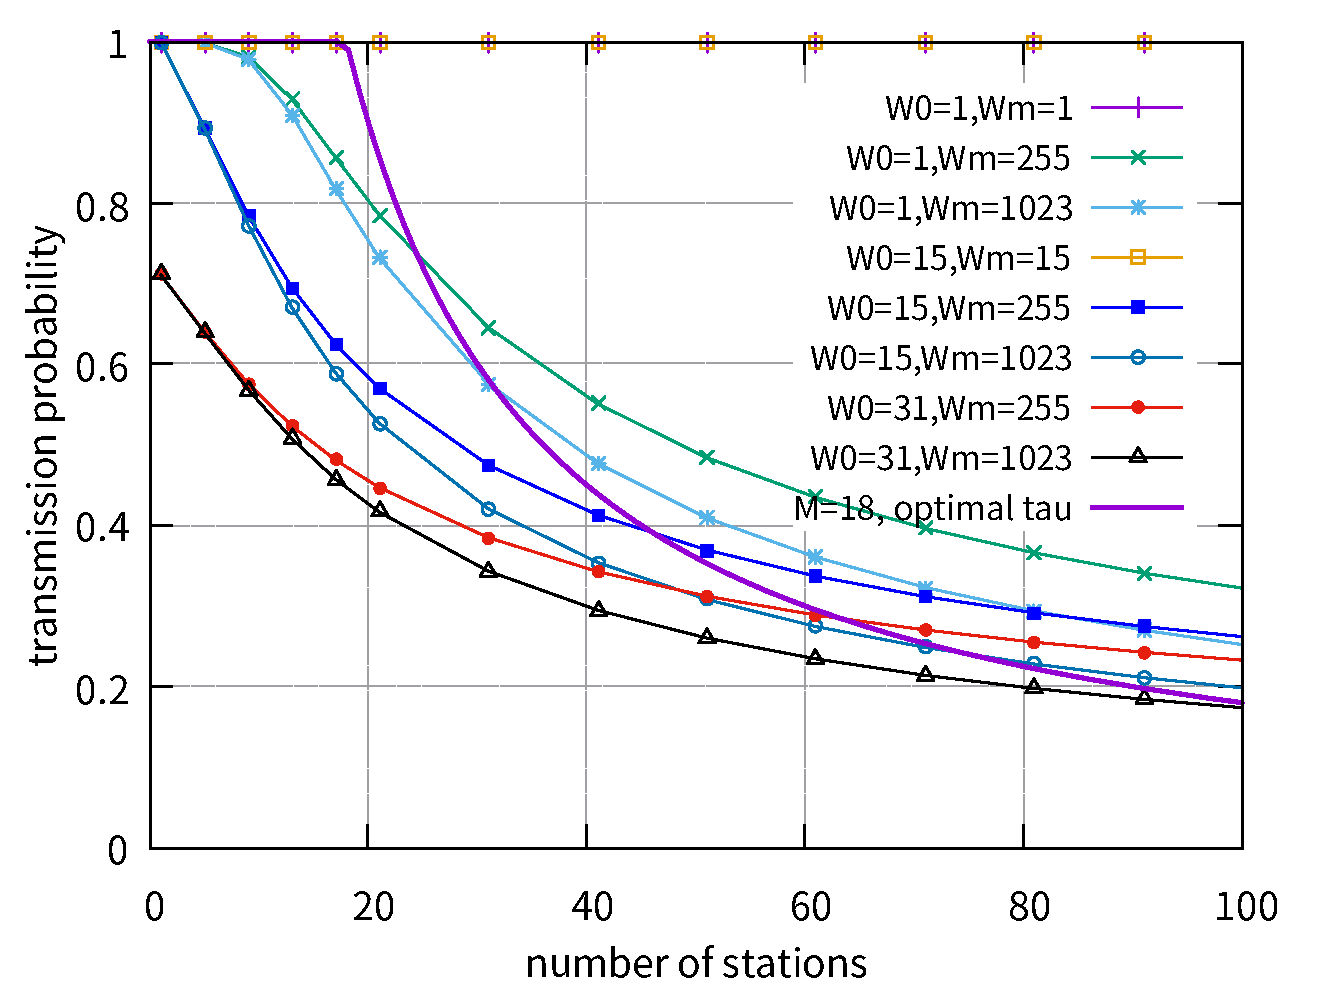
\includegraphics[scale=.38]{./figure/Section_perf_eval/tau/n_tau_perf_M18_x100.pdf}
\caption{Case 2, given $M=18$}
\label{fig_tau_n_M18_detail}
\end{subfigure}

\caption{Details of transmission probability versus number of stations when $n\leq 100$}
\label{fig_tau_n_detail}
\end{figure}

Then, two subfigures as in Fig. \ref{fig_tau_n_detail} are generated from Fig. \ref{fig_tau_n} with $n$ ranges from $[0,100]$ to observe practical scenarios more clearly. 
Another observation whereby is that when $W_0=1$, line of $\tau$ will have a flat start, which happens to match better with $\tau^\star$ at $n\leq M$.

All above observations are summed up that $W_0$ has significant influence on scenario of $n\leq M$, while $W_m$ counts when $n$ is large, namely the dense scenario. 
In the next two subsections, the system efficiency and access delay under different parameter configurations are practically evaluated, whereby above observed effects of parameters could be conformed.



\subsubsection{Configure $OCW_{max}$}

\begin{figure}[!t]
\centering
\begin{subfigure}{0.5\textwidth}  
  \centering  
  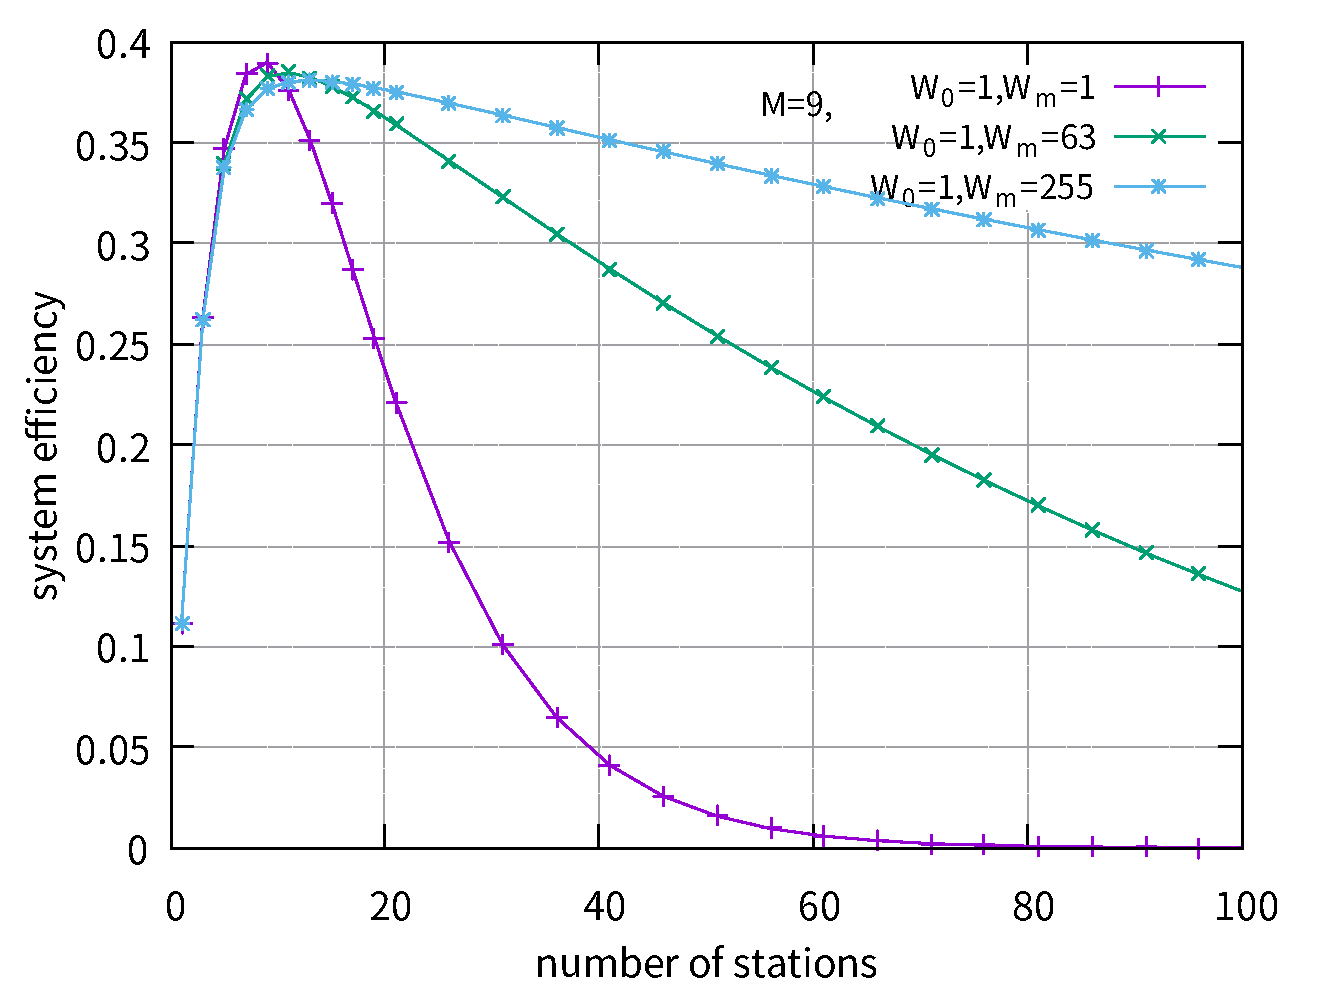
\includegraphics[scale=0.38]{./figure/Section_perf_eval/W0/n_eff_perf_W01.pdf}  
    \caption{System efficiency versus number of stations}   
    \label{fig_n_eff_Wm}
\end{subfigure}   

\begin{subfigure}{0.5\textwidth}
	\centering
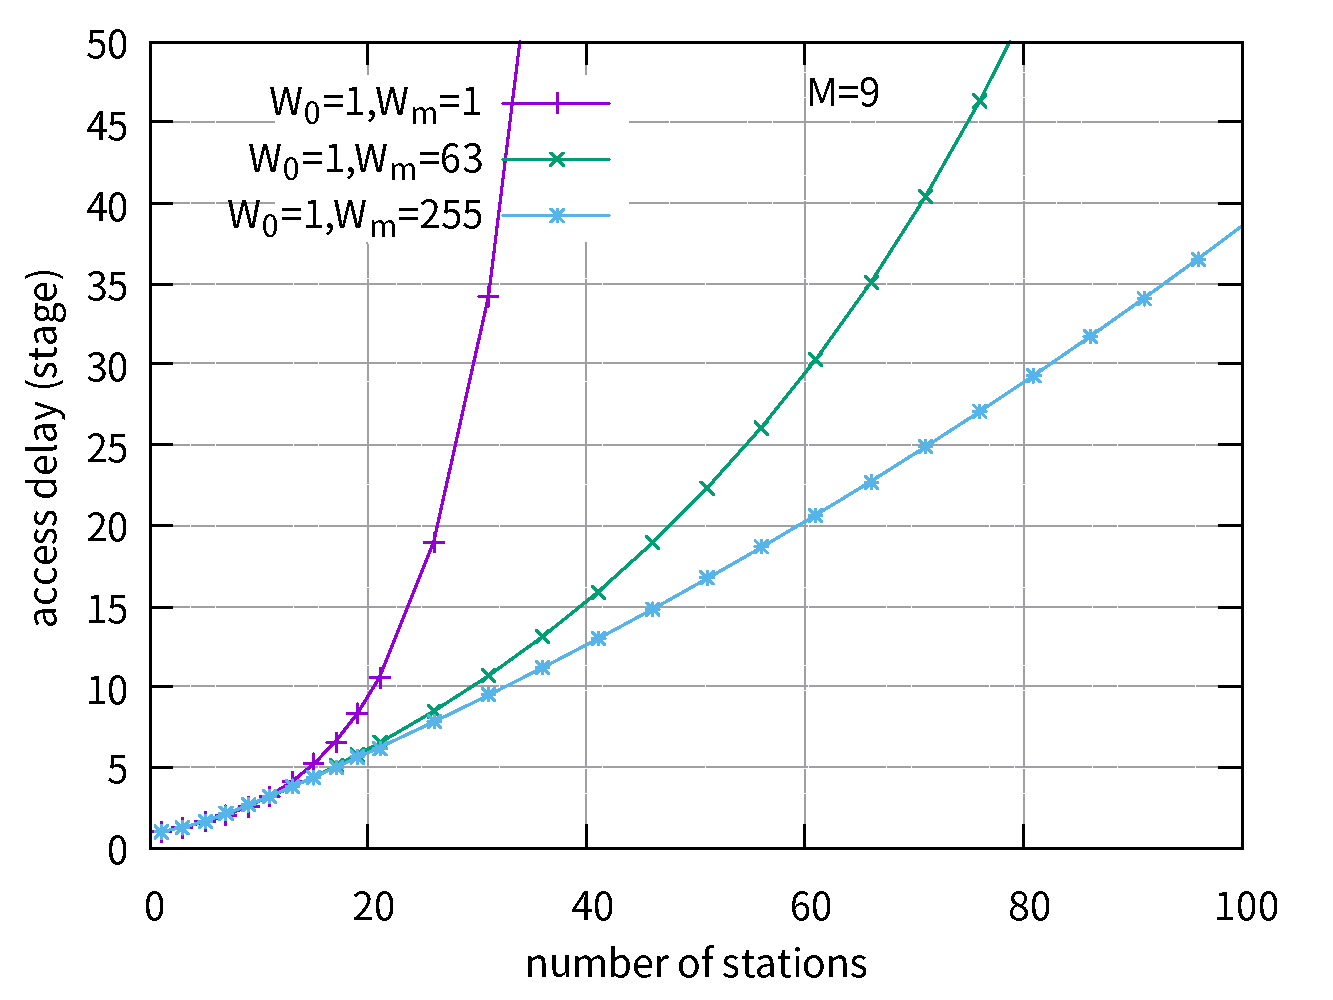
\includegraphics[scale=.38]{./figure/Section_perf_eval/W0/n_delay_perf_W01.pdf}
\caption{Access delay versus number of stations}
\label{fig_n_delay_Wm}
\end{subfigure}
\caption{Example of Configuring $OCW_{max}$, given $M=9$}
\label{fig_Wm}
\end{figure}

With above rough rules, the effect of $OCW_{max}$ is first evaluated by setting different $OCW_{max}$ while fixing $OCW_{min}=1$ and $M=9$.
In Fig. \ref{fig_n_eff_Wm}, three cases which has the same $OCW_{min}$ are selected to clearly display the effect of $OCW_{max}$ on system efficiency.
From the figure, it is evident that larger $OCW_{max}$ is much better for system efficiency when $n\geq M$. 
The result corresponds to the above rules obtained from the effect of parameters on $\tau$.
Additionally, larger $OCW_{max}$ results in shorter access delay. 
%And since we use the same data with that in figure \ref{fig_tau_n_M9}, we find that the lines which converge in figure \ref{fig_tau_n_M9} also have the same tendency in figure \ref{fig_n_delay_Wm}. 


\subsubsection{Configure $OCW_{min}$}

\begin{figure}[!t]
\centering
\begin{subfigure}{0.5\textwidth}  
  \centering  
  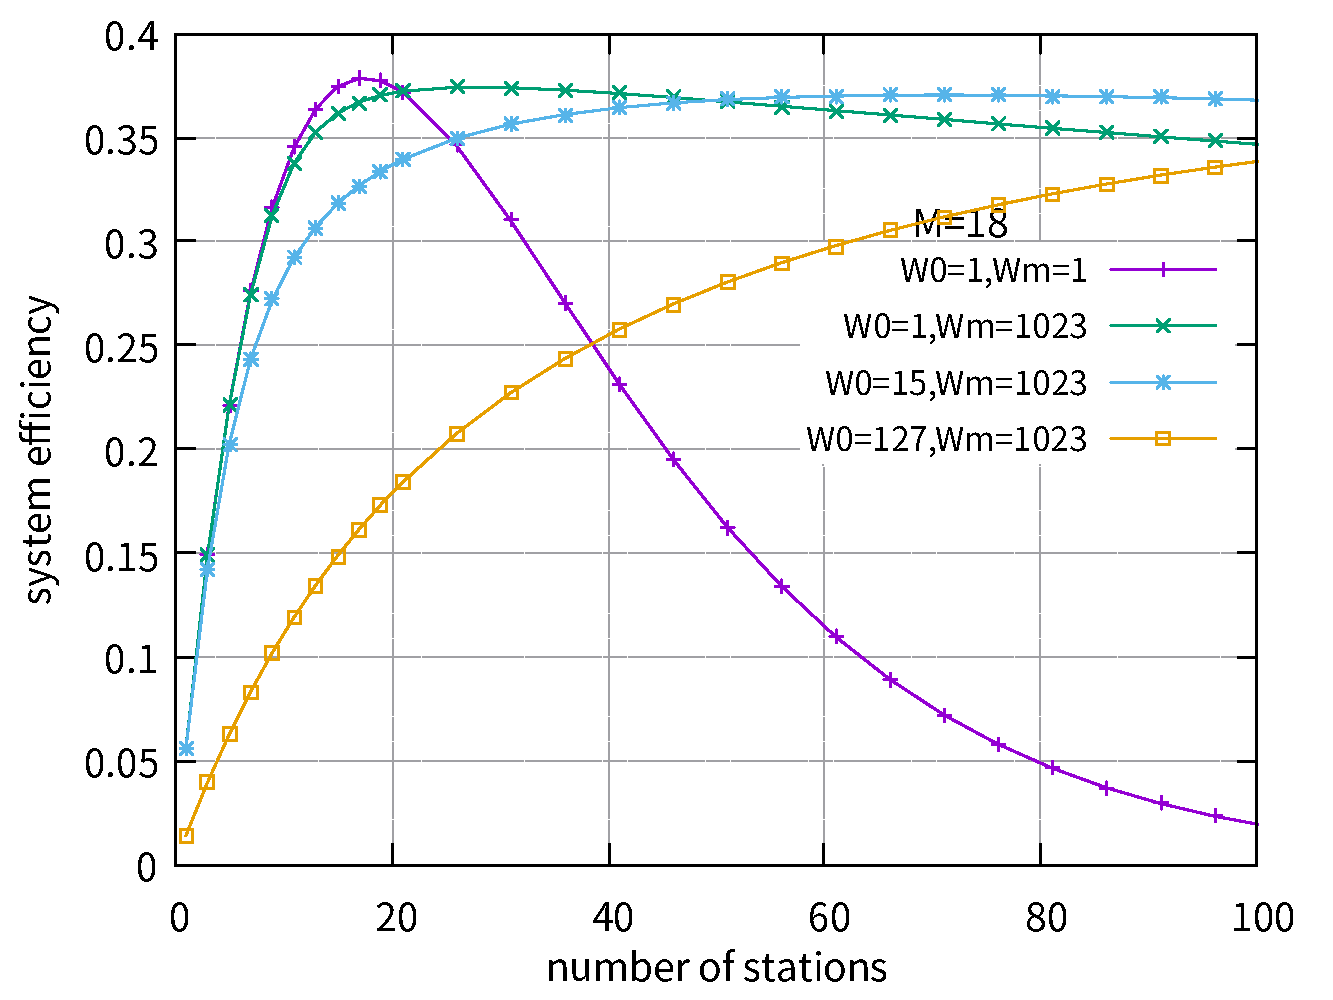
\includegraphics[scale=0.38]{./figure/Section_perf_eval/Wm/n_eff_perf_Wm1023.pdf}  
    \caption{System efficiency versus number of stations}   
    \label{fig_n_eff_W0}
\end{subfigure}   

\begin{subfigure}{0.5\textwidth}
	\centering
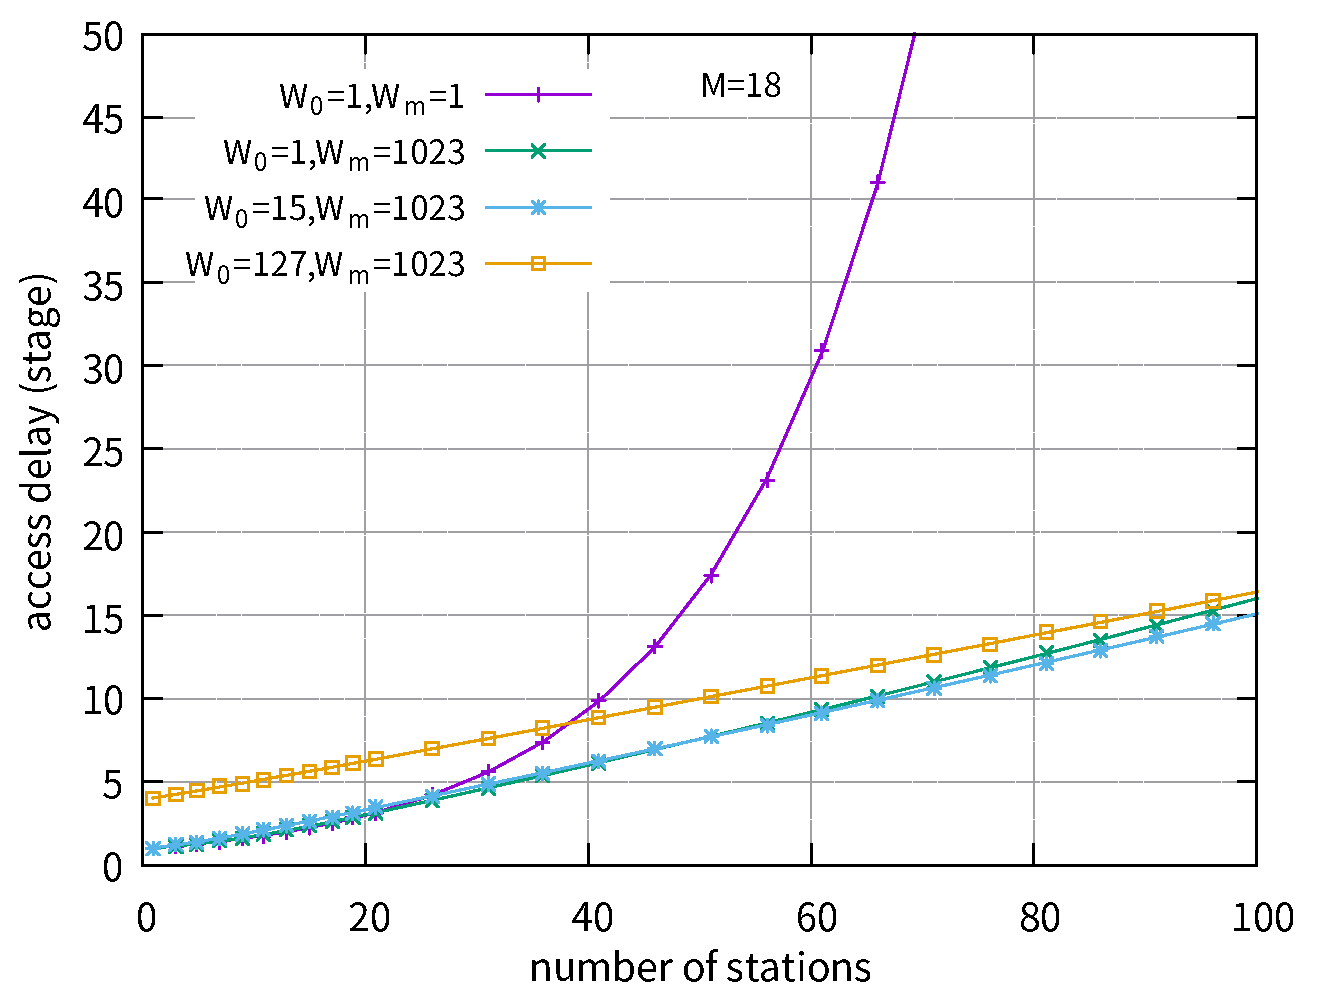
\includegraphics[scale=.38]{./figure/Section_perf_eval/Wm/n_delay_perf_Wm1023.pdf}
\caption{Access delay versus number of stations}
\label{fig_n_delay_W0}
\end{subfigure}
\caption{Example of Configuring $OCW_{min}$, given $M=18$}
\label{fig_W0}
\end{figure}

To estimate the effect of $OCW_{min}$, the performance of different configurations of $OCW_{min}$ while fixing large $OCW_{max}=1023$, and $M=18$. 
First, $OCW_{min}$ determines the start of the probability $\tau$, and it has a significant influence on the scenario of $n\leq M$.
From Fig. \ref{fig_n_eff_W0} and \ref{fig_n_delay_W0}, we find larger $OCW_{min}=127$ has lower system efficiency and larger access delay. 
Secondly, as stated in Section \ref{contend_window} that $W_0=W_m\leq M$ is the perfect configuration in the scenario of $n\leq M$, it is validated in Fig. \ref{fig_W0} that maximum system efficiency and minimum access delay are achieved with the configuration in the scenario of $n\leq M$.
However, the configuration of small $OCW_{min}$ and large $OCW_{max}$ almost achieves as good performance as the perfect configuration.  

To this end, all observed rules are listed as follows.
 
\begin{itemize}
\item[1] For $M$: the larger the better
\item[2] For $OCW_{min}, OCW_{max}$:
	\begin{itemize}
	\item $OCW_{min}$ counts when $n\leq M$. Smaller $OCW_{min}$ is better.
	\item $OCW_{max}$ counts when $n>M$. Larger $OCW_{max}$ is better.
	\end{itemize}
\end{itemize}
\begin{itemize}
	\item Special case: for $n\leq M$\\
	$OCW_{max}=OCW_{min}<M$ is the optimal configuration.  
\end{itemize}





\section{Conclusion}   \label{sec_conclu}
In this paper, Bianchi's Markov chain model is extended for saturation analysis of the OFDMA-based MCRA mechanism of 802.11ax.
The simple Markov chain model is validated that it could precisely depict the steady state behavior of OFDMA-based MCRA of 802.11ax.
Thereby, closed-form expressions of system efficiency and access delay are derived. 
Finally, it is observed that performance strongly depends on the system parameters. 
Larger number of RUs or subchannels for random access results in more successful contending stations at a stage.
The initial contention window counts when only a few stations exist, while maximum contention window has significant influence in the dense scenario.

Different from DCF of legacy 802.11, the OFDMA-based MCRA mechanism is more flexible, with system parameters dynamically configured.
A real-time algorithm is required to configure the system parameters dynamically. 
This paper takes the first step to catch some insight from the steady state behavior of the MCRA mechanism.
In the future, transient analysis is necessary to generate a configuration algorithm.

%An interesting result is that the maximum system efficiency and minimum access delay are obtained by the same transmission probability $\tau$, which is given by $\tau^\star = min \lbrace 1,M/n\rbrace$. 
%Then rules of configuration of parameter set aimed at reaching the optimal transmission probability $\tau^\star$ is proposed for AP according to system state, mainly the number of contending stations. 
%The last group cases of various parameter sets validates our proposed rules.

%We find an interesting result that system efficiency and access delay behave consistent with each other and they both strongly depend on the system parameters.
%Larger $M$ is better whenever $n$ is large or small.
%Smaller $OCW_{min}$ is better and affects more in case when $n$ is small.
%Larger $OCW_{max}$ is better and affcets more in case when $n$ is large. 
%Especially, an optimal configuration $OCW_{min}=OCW_{max}\leq M$ fits in case $n\leq M$. 
%All above are the rough insight we obtain from steady state behavior.
%To generate a dynamic algorithm to configure the system parameters requires transient analysis, which could be done in the future.

% An example of a floating figure using the graphicx package.
% Note that \label must occur AFTER (or within) \caption.
% For figures, \caption should occur after the \includegraphics.
% Note that IEEEtran v1.7 and later has special internal code that
% is designed to preserve the operation of \label within \caption
% even when the captionsoff option is in effect. However, because
% of issues like this, it may be the safest practice to put all your
% \label just after \caption rather than within \caption{}.
%
% Reminder: the "draftcls" or "draftclsnofoot", not "draft", class
% option should be used if it is desired that the figures are to be
% displayed while in draft mode.
%
%\begin{figure}[!t]
%\centering
%\includegraphics[width=2.5in]{myfigure}
% where an .eps filename suffix will be assumed under latex, 
% and a .pdf suffix will be assumed for pdflatex; or what has been declared
% via \DeclareGraphicsExtensions.
%\caption{Simulation results for the network.}
%\label{fig_sim}
%\end{figure}

% Note that the IEEE typically puts floats only at the top, even when this
% results in a large percentage of a column being occupied by floats.


% An example of a double column floating figure using two subfigures.
% (The subfig.sty package must be loaded for this to work.)
% The subfigure \label commands are set within each subfloat command,
% and the \label for the overall figure must come after \caption.
% \hfil is used as a separator to get equal spacing.
% Watch out that the combined width of all the subfigures on a 
% line do not exceed the text width or a line break will occur.
%
%\begin{figure*}[!t]
%\centering
%\subfloat[Case I]{\includegraphics[width=2.5in]{box}%
%\label{fig_first_case}}
%\hfil
%\subfloat[Case II]{\includegraphics[width=2.5in]{box}%
%\label{fig_second_case}}
%\caption{Simulation results for the network.}
%\label{fig_sim}
%\end{figure*}
%
% Note that often IEEE papers with subfigures do not employ subfigure
% captions (using the optional argument to \subfloat[]), but instead will
% reference/describe all of them (a), (b), etc., within the main caption.
% Be aware that for subfig.sty to generate the (a), (b), etc., subfigure
% labels, the optional argument to \subfloat must be present. If a
% subcaption is not desired, just leave its contents blank,
% e.g., \subfloat[].


% An example of a floating table. Note that, for IEEE style tables, the
% \caption command should come BEFORE the table and, given that table
% captions serve much like titles, are usually capitalized except for words
% such as a, an, and, as, at, but, by, for, in, nor, of, on, or, the, to
% and up, which are usually not capitalized unless they are the first or
% last word of the caption. Table text will default to \footnotesize as
% the IEEE normally uses this smaller font for tables.
% The \label must come after \caption as always.
%
%\begin{table}[!t]
%% increase table row spacing, adjust to taste
%\renewcommand{\arraystretch}{1.3}
% if using array.sty, it might be a good idea to tweak the value of
% \extrarowheight as needed to properly center the text within the cells
%\caption{An Example of a Table}
%\label{table_example}
%\centering
%% Some packages, such as MDW tools, offer better commands for making tables
%% than the plain LaTeX2e tabular which is used here.
%\begin{tabular}{|c||c|}
%\hline
%One & Two\\
%\hline
%Three & Four\\
%\hline
%\end{tabular}
%\end{table}


% Note that the IEEE does not put floats in the very first column
% - or typically anywhere on the first page for that matter. Also,
% in-text middle ("here") positioning is typically not used, but it
% is allowed and encouraged for Computer Society conferences (but
% not Computer Society journals). Most IEEE journals/conferences use
% top floats exclusively. 
% Note that, LaTeX2e, unlike IEEE journals/conferences, places
% footnotes above bottom floats. This can be corrected via the
% \fnbelowfloat command of the stfloats package.





% if have a single appendix:
%\appendix[Proof of the Zonklar Equations]
% or
%\appendix  % for no appendix heading
% do not use \section anymore after \appendix, only \section*
% is possibly needed

% use appendices with more than one appendix
% then use \section to start each appendix
% you must declare a \section before using any
% \subsection or using \label (\appendices by itself
% starts a section numbered zero.)
%


\appendices
%\section{Proof of the First Zonklar Equation}
%Appendix one text goes here.

% you can choose not to have a title for an appendix
% if you want by leaving the argument blank
%\section{}
%Appendix two text goes here.


% use section* for acknowledgment
%\section*{Acknowledgment}


%The authors would like to thank...


% Can use something like this to put references on a page
% by themselves when using endfloat and the captionsoff option.
\ifCLASSOPTIONcaptionsoff
  \newpage
\fi



% trigger a \newpage just before the given reference
% number - used to balance the columns on the last page
% adjust value as needed - may need to be readjusted if
% the document is modified later
%\IEEEtriggeratref{8}
% The "triggered" command can be changed if desired:
%\IEEEtriggercmd{\enlargethispage{-5in}}

% references section

% can use a bibliography generated by BibTeX as a .bbl file
% BibTeX documentation can be easily obtained at:
% http://mirror.ctan.org/biblio/bibtex/contrib/doc/
% The IEEEtran BibTeX style support page is at:
% http://www.michaelshell.org/tex/ieeetran/bibtex/
\bibliographystyle{IEEEtran}
% argument is your BibTeX string definitions and bibliography database(s)
\bibliography{formula.bib}
%
% <OR> manually copy in the resultant .bbl file
% set second argument of \begin to the number of references
% (used to reserve space for the reference number labels box)
%\begin{thebibliography}{1}

%\bibitem{IEEEhowto:kopka}
%H.~Kopka and P.~W. Daly, \emph{A Guide to \LaTeX}, 3rd~ed.\hskip 1em plus
%  0.5em minus 0.4em\relax Harlow, England: Addison-Wesley, 1999.

%\end{thebibliography}

% biography section
% 
% If you have an EPS/PDF photo (graphicx package needed) extra braces are
% needed around the contents of the optional argument to biography to prevent
% the LaTeX parser from getting confused when it sees the complicated
% \includegraphics command within an optional argument. (You could create
% your own custom macro containing the \includegraphics command to make things
% simpler here.)
%\begin{IEEEbiography}[{\includegraphics[width=1in,height=1.25in,clip,keepaspectratio]{mshell}}]{Michael Shell}
% or if you just want to reserve a space for a photo:

\begin{IEEEbiography}{Michael Shell}
Biography text here.
\end{IEEEbiography}

% if you will not have a photo at all:
\begin{IEEEbiographynophoto}{John Doe}
Biography text here.
\end{IEEEbiographynophoto}

% insert where needed to balance the two columns on the last page with
% biographies
%\newpage

\begin{IEEEbiographynophoto}{Jane Doe}
Biography text here.
\end{IEEEbiographynophoto}

% You can push biographies down or up by placing
% a \vfill before or after them. The appropriate
% use of \vfill depends on what kind of text is
% on the last page and whether or not the columns
% are being equalized.

%\vfill

% Can be used to pull up biographies so that the bottom of the last one
% is flush with the other column.
%\enlargethispage{-5in}



% that's all folks
\end{document}


